\documentclass[11pt]{article}
\usepackage[margin=1in]{geometry}
\usepackage[T1]{fontenc}
\usepackage{lmodern}
\usepackage{microtype}
\usepackage{amsmath,amssymb}
\usepackage{booktabs}
\usepackage{array}
\usepackage{graphicx}
\usepackage[authoryear,round]{natbib}
\usepackage{caption}
\usepackage[section]{placeins}
\usepackage{xcolor}
\definecolor{darkblue}{rgb}{0.0,0.2,0.55}
\usepackage[colorlinks=true,citecolor=darkblue,urlcolor=darkblue,linkcolor=black]{hyperref}
\captionsetup{font=small,labelfont=bf}
\setlength{\parskip}{0.5em}
\setlength{\parindent}{0pt}
\setlength{\emergencystretch}{2em}
\newcolumntype{L}[1]{>{\raggedright\arraybackslash}p{#1}}

\title{How Will Paid AI Spread? Evidence from Home Computers in US Households, 1984--2013\\[0.4em]
\large A test of the profit switch hypothesis with US household surveys and computer price indexes}
\author{}
\date{11 November 2026}

\begin{document}
\maketitle

\begin{abstract}
\noindent The spread of home computers through US households is a guide to how paid AI may spread. We study that spread with 178{,}891 households interviewed in the Consumer Expenditure Survey from January 1994 to March 2013, the Bureau of Economic Analysis computer price index, and, for the years back to 1984, 369{,}393 households in eight Current Population Survey supplements from October 1984 to October 2003. Our findings cover 1994 to 2012, since 2012 is the last full year of Consumer Expenditure Survey data. Over those years the share of US households that owned a computer rose from 24\% to 81\%. We find three key results. First, falling quality-adjusted computer prices, far more than rising incomes, paced that rise. Falling prices account for 53 of its 57 percentage points and rising household spending for 3, even though the median price paid for a computer fell only 7\% from 1994 to 2012. Second, the gap in computer ownership between the richest and poorest fifths of households, ranked by income, widened from 39 percentage points in 1994 to 54 in 2003, then narrowed to 37 in 2012. Every household faced the same computer price, but a price cut is most likely to tip households close to affording a computer into buying one, and the households close to affording one were richer households in the 1990s and poorer households in the 2000s. Third, falling prices left the education gap in computer ownership in place. The gap between households headed by college and high-school graduates grew from 30 percentage points in 1994 to 39 in 1997 and narrowed only after 2001, once most college households owned a computer, and among households with equal spending it did not narrow from 1994 to 2012. If paid AI follows this pattern, policymakers will need a quality-adjusted price index for AI services to track how affordable AI is becoming. Once most households pay for AI, a given income gain would raise paid AI use most if it went to the bottom half of households, but cheaper AI alone may leave more educated households ahead.
\end{abstract}

\clearpage
\section*{Summary of core findings}

\noindent The spread of home computers through US households is a guide to how paid AI may spread. Once a technology reaches 20--30\% of households, affordability (what households can spend relative to its price) should pace its further spread. We test this hypothesis on the home computer with 178{,}891 households interviewed in the Consumer Expenditure Survey from January 1994 to March 2013, the Bureau of Economic Analysis price index for personal computers, and, for the years back to 1984, 369{,}393 households in eight Current Population Survey supplements from October 1984 to October 2003. The findings below come from the Consumer Expenditure Survey and run from 1994 to 2012, its last full year of data.

\noindent We find that falling quality-adjusted computer prices, far more than rising incomes, paced the spread of home computers, first among rich households and then among poorer ones, but left the education gap in computer ownership in place.
\begin{enumerate}\setlength{\itemsep}{1pt}
\item \textbf{Falling quality-adjusted computer prices, far more than rising incomes, paced the spread of computers.} Of the rise in the share of US households that owned a computer, from 24\% in 1994 to 81\% in 2012, our model attributes 53 percentage points to the falling quality-adjusted computer price (the price of a computer of fixed capability) and 3 points to rising household spending after inflation. Across the 20 years from 1994 to 2013, the spending threshold, the yearly spending at which a household was more likely than not to own a computer, fell by 4--6\% for each 10\% fall in the quality-adjusted price, only about half the 10\% that affordability alone predicts. But from 1994 to 2012 the quality-adjusted price fell 98\%, while the dollar price that households paid for a computer fell by only 7\% at the median, because the gains in technology went into better computers and into \emph{productization}, the work of turning the computer into a product that ordinary households could buy and use.
\item \textbf{As computer prices fell, the gap in computer ownership between rich and poor households widened and then narrowed.} The gap between the richest and poorest fifths of households, ranked by income, grew from 39 percentage points in 1994 to 54 in 2003, then fell to 37 in 2012, slightly below its 1994 level. Every household faced the same computer price, but a price cut is most likely to tip households close to affording a computer into buying one. These were the richest households in 1994 and poorer households after 2003, when most rich households owned one.
\item \textbf{Falling computer prices over time still left the education gap in computer ownership in place.} The computer ownership gap between households headed by college and high-school graduates grew from 30 percentage points in 1994 to 39 in 1997 and narrowed only after 2001, once more than 80\% of college households owned a computer. Averaged over 1994--2012, a household headed by a college graduate that spent \$10{,}000 a year was as likely to own a computer as an otherwise similar household headed by a high-school graduate that spent \$28{,}000, and this multiple of 2.8 did not shrink as computer prices fell.
\end{enumerate}
\noindent If paid AI follows the same pattern, better AI at the same subscription price may do far more than income growth to spread it, so policymakers will need a quality-adjusted price index for AI services to track how affordable AI is becoming. Once most households pay for AI, a given income gain would raise paid AI use most if it went to the bottom half of households, but cheaper AI alone may leave more educated households ahead.

\clearpage

\section{Introduction}

Home computers spread to most US households between 1984 and 2012, while computers became far cheaper for what they could do and household incomes rose only modestly. In 1984, 8\% of US households owned a computer, according to the Current Population Survey, and by 2012, 81\% did, according to the Consumer Expenditure Survey. From 1994 to 2012 alone, the \emph{quality-adjusted price} of a personal computer, which is the price of a computer of fixed capability, fell to 1/56 of its 1994 level, while the median household's spending rose by 61\% in current dollars and by 14\% after inflation. This paper asks which of these two changes, falling computer prices or rising household incomes, paced the spread of home computers, and how the two worked together.

The answer bears on how paid artificial intelligence (AI) services may spread through households. Generative AI has spread faster than the personal computer did. In August 2025, less than three years after the release of ChatGPT, 54.6\% of US adults aged 18 to 64 used generative AI. In 1984, three years after the IBM PC went on sale, 19.7\% of US adults aged 18 to 64 used a personal computer \citep{bick2025state}. Households pay nothing in dollars for much of the use of generative AI. If paid AI services follow the pattern of home computers, the history of the home computer can show which households may take up paid AI as its price falls, and when.

The answer also bears on the \emph{profit switch hypothesis}, which holds that what paces the spread of a new technology in the country that invents it changes as the technology spreads. Until about 20--30\% of households have adopted the technology, firms' profit share, the share of national income that goes to profits, paces the spread through the investment that lowers the cost of making the technology. After that point, \emph{affordability}, meaning what households can spend relative to the price of the technology, paces the spread. The personal computer was developed and first sold in volume in the United States, and US household surveys record computer ownership from 1984, so US home computers make a natural first test of the hypothesis.

In this paper, we use two US household surveys that together cover 1984 to 2013. The Consumer Expenditure Survey (CE) of the Bureau of Labor Statistics records computer ownership and spending for 178{,}891 households interviewed from January 1994 to March 2013, and all of our main findings come from the CE. Because the 2013 CE files cover only January to March, we measure changes from 1994 to 2012, years in which the share of US households that owned a computer, which we call the \emph{computer ownership rate}, rose from 24\% to 81\%. The Current Population Survey (CPS) records computer ownership and family income for 369{,}393 households in eight supplements from October 1984 to October 2003, and only the CPS covers the years before the computer ownership rate reached 20\%. We measure each household's income by its \emph{long-run spending}, the household's average spending across its survey interviews at an annual rate, which predicts computer ownership better than reported income does in every year from 1994 to 2012.

We test affordability by asking whether the spending a household needed before it owned a computer fell in step with the quality-adjusted computer price. For each year from 1994 to 2013 we estimate the \emph{spending threshold}, the level of long-run spending at which a household with average location and traits has a 50\% chance of owning a computer, and we then regress the 20 yearly spending thresholds on the quality-adjusted computer price. Under \emph{pure affordability}, the computer price and household spending are all that matter for whether a household owns a computer. When the computer price halves, the spending a household needs before it buys a computer also halves, so in a regression of the log spending threshold on the log computer price and a time trend, the coefficient on the log computer price is 1 and the coefficient on the time trend is 0 (Section~\ref{sec:model}). We call the first coefficient, $b$, the \emph{price effect} and the second, $d$, the \emph{unexplained trend}.

We estimate one baseline regression and extend it in two directions. The baseline regression uses observed long-run spending and the household's state or region. The extended regression corrects long-run spending for noise between interviews and adds household traits and the education of the household head, and the CPS extension reaches back to 1984 to test whether the unexplained trend changed when the computer ownership rate passed 20--30\%.

Our main finding is that from 1994 to 2012 falling quality-adjusted computer prices, far more than rising household incomes, paced the spread of home computers, first among rich households and then among poorer ones, but left the education gap in computer ownership in place.

First, \textbf{falling computer prices did almost all the work of spreading home computers from 1994 to 2012.} In constant dollars, our model attributes 53 percentage points of the 57-point rise in the computer ownership rate from 1994 to 2012 (94\% of the part that prices and incomes explain) to the falling computer price and 3 points (6\%) to rising household spending. Falling prices did this much even though the spending threshold followed the quality-adjusted computer price at only about half the strength that pure affordability predicts (Figure~\ref{fig:tau}). Our estimates imply that, across the 20 years from 1994 to 2013, a 10\% fall in the quality-adjusted computer price lowered the spending threshold by 4.6\% in the baseline regression ($b = 0.45$) and by 6.0\% in the extended regression ($b = 0.59$). Both 90\% intervals for $b$ exclude 1, the value that pure affordability predicts, while the estimated unexplained trend lies within half a percent a year of zero, as pure affordability also predicts. Half strength was enough because from 1994 to 2012 the computer price relative to all consumer prices fell to 1/79 of its 1994 level, while median long-run spending rose by only 14\% after inflation.

The price that fell was the quality-adjusted price, which fell because each dollar bought a better computer. From 1994 to 2012 the dollar price that households paid for a computer fell by 7\% at the median and by about half at the 90th percentile, while the quality-adjusted computer price fell 98\%. Better computers account for 84--98\% of the 1994--2012 fall in the quality-adjusted price, measured in logs, and lower dollar prices account for the rest. The dollar price fell far less because the gains in technology went into better computers and into \emph{productization}, the work of turning the computer into a product that ordinary households could buy and use. Measured against the dollar price, affordability explains almost none of the spread of computers from 1994 to 2012.

Second, as computer prices fell, \textbf{the gap in computer ownership between rich and poor households widened and then narrowed}. In the raw survey data, the gap between the computer ownership rates of the richest and poorest fifths of households, ranked by reported income, grew from 39 percentage points in 1994 to 54 in 2003 and fell to 37 in 2012, slightly below its 1994 level. Every household faced the same computer price, but in the household model (Figure~\ref{fig:interaction}) a price cut is most likely to tip households whose spending is near the spending threshold into buying a computer. In 1994 the spending threshold was above the spending of 95\% of households, so the households close to buying a computer were among the highest spenders. By 2012 the spending threshold was below the spending of 96\% of households, so the households close to buying were among the lowest spenders.

Third, \textbf{falling computer prices still left the education gap in computer ownership in place.} In the raw survey data, the gap between the computer ownership rates of households headed by college graduates and households headed by high-school graduates grew from 30 percentage points in 1994 to 39 in 1997 and narrowed only after 2001, once more than 80\% of college households owned a computer. Pure affordability rules out any education gap among households with the same spending, yet averaged over 1994--2012, a household headed by a college graduate that spent \$10{,}000 a year was as likely to own a computer as an otherwise similar household headed by a high-school graduate that spent \$28{,}000, and this multiple of 2.8 did not shrink as computer prices fell (Figure~\ref{fig:educ}).

These estimates hold up in robustness checks. Fitting the extended regression's two stages as one Bayesian model of all 178{,}891 CE households of 1994--2013 gives $b = 0.60$, against 0.59 from the two stages, and most other choices of sample, spending measure, and link function leave $b$ between 0.37 and 0.61 (Section~\ref{sec:robust}).

Our approach builds on threshold models of the spread of durable goods, such as cars and refrigerators, in which a falling threshold passes down through the income distribution \citep{david1969,bonus1973,geroski2000}, and on \citet{griliches1957}, who showed that the profitability of hybrid corn explains how fast and how far hybrid corn spread across US states. We estimate the spending threshold directly in each year and test its path against an explicit benchmark, $b = 1$ and $d = 0$, that the data can reject. \citet{greenwood2005} argue that technical progress lowered the prices of household appliances and spurred their adoption, and they note that poor households bought durable goods later than rich households, when prices were lower. We measure how much of the spread of home computers came from falling prices and how much from rising incomes, and we show how the households that a price cut helps most, those close to affording a computer, moved down the income distribution. Hedonic price indexes adjust the price of a computer for its quality \citep{berndt2001,pakes2003}, and measures based on computing performance show larger price falls than the official indexes \citep{nordhaus2007}. We show that from 1994 to 2012 the spread of home computers followed the quality-adjusted computer price, at about half strength, while the dollar price that households paid barely fell.

Our estimates also bear on earlier work about how income, education, and spillovers among computer users shape who owns a computer. \citet{chinn2007} find that differences in income account for most of the gap in computer and internet use across countries. \citet{nelson1966} argued that education speeds the adoption of new technology, and \citet{riddell2017} find that more schooling raises the chance that a worker uses a computer on the job. \citet{goolsbee2002} find that US households were more likely to buy a first home computer in areas where more households already owned one, which is evidence of spillovers from learning or from networks of computer users. Spillovers that grew with national computer ownership would show up in our regressions as a negative unexplained trend, and we find no such trend in the national series for 1994 to 2013, although 20 yearly estimates cannot rule out small trends. The paper also gives a household-level test of the affordability phase of the profit switch hypothesis, which companion work studies with cross-country data on internet adoption.

The estimates show how closely the spending threshold followed the computer price, but the data limit what the estimates can say about causes and about the early years of the spread of computers. The computer price is the same for every household in a given year, so $b$ and $d$ rest on the 20 yearly spending thresholds of 1994--2013, and they also pick up anything else that moved with computer prices over time, such as the spread of the internet and of software. The household data can measure how much of the fall in the spending threshold the computer price leaves unexplained, but the household data cannot say what caused that unexplained part. The surveys also cannot test whether the forces behind computer ownership changed at 20--30\% ownership, because only two surveys, the CPS of 1984 and 1989, measure computer ownership below 20\% (Appendix~\ref{sec:cps}).

If paid AI services follow the pattern that home computers followed after 1994 (Section~\ref{sec:ai}), policymakers will need a quality-adjusted price index for AI services to track how affordable AI is becoming, because the subscription price, like the dollar price of a computer, may fall far less than the quality-adjusted price. Every household would face the same price for an AI service, but a cut in that price would be most likely to tip households close to affording paid AI into paying for it, so the gap in paid AI use between rich and poor households may widen before it narrows. Once most households pay for AI, a given income gain would raise paid AI use most if it went to the bottom half of households, but cheaper AI alone may leave more educated households ahead. These implications hold only for AI that households pay for in dollars. Firms can also earn from free AI indirectly, through advertising, which OpenAI said in January 2026 it would test in the free tier of ChatGPT \citep{openai2026}, and through the conversations that users allow firms to use to train their models \citep{anthropic2025}. How far AI funded in these ways spreads may depend more on what firms earn from it than on what households can spend. To test the profit switch hypothesis for AI, statistical agencies would also need a household survey that records AI use, paid or free, and income every year from early adoption on.

Section~\ref{sec:model} sets out a household model of computer ownership and derives what pure affordability predicts. Sections~\ref{sec:data} and~\ref{sec:method} describe the data and the method, Section~\ref{sec:findings} presents the findings, Section~\ref{sec:discussion} discusses them, and Section~\ref{sec:ai} draws out the implications for AI diffusion and policy. The appendices give details of the data and the method, the estimates in tables, and the robustness checks.

\section{A household model of computer ownership}
\label{sec:model}

This section sets out when a household owns a computer, derives what pure affordability predicts, and shows how the computer price and household income interact. Section~\ref{sec:method} turns the household model into the regressions we estimate.

\subsection{When a household owns a computer}

Household $i$ owns a computer in year $t$ if the household's long-run spending, relative to the cost of owning a computer, exceeds a cutoff:
\begin{equation}
\ln s_{it} - \ln K_t > c_i, \qquad c_i \sim \text{Normal}(c, \sigma^2),
\label{eq:rule}
\end{equation}
where $s_{it}$ is the household's long-run spending in current dollars a year and $K_t$ is the cost of owning a computer in year $t$, in current dollars. The cutoff $c_i$ is the amount, in logs, by which the household's spending must exceed the cost of owning a computer before the household buys a computer. The mean cutoff across households is $c$, and the standard deviation of cutoffs across households is $\sigma$, also in logs. A household that values a computer highly has a low cutoff. We write $x_{it} = \ln s_{it}$ for the household's log long-run spending. The probability that a household with log spending $x_{it}$ owns a computer is
\begin{equation}
\Pr(\text{own}_{it} = 1 \mid x_{it}) = \Phi\!\left(\frac{x_{it} - \tau_t}{\sigma}\right), \qquad \tau_t = c + \ln K_t,
\label{eq:prob}
\end{equation}
where $\Phi$ is the standard normal distribution function. The spending threshold $\tau_t$ is the log long-run spending at which the probability of owning a computer is one half. A household whose spending is above the spending threshold is more likely than not to own a computer, and a household whose spending is below the spending threshold is less likely than not to own a computer. The computer ownership rate, the share of households that own a computer, is
\begin{equation}
P_t = \int \Phi\!\left(\frac{x - \tau_t}{\sigma}\right) dF_t(x),
\label{eq:diffusion}
\end{equation}
where $F_t$ is the distribution of log long-run spending across households in year $t$. Equations \eqref{eq:rule}--\eqref{eq:diffusion} are the threshold model of durable-good ownership \citep{bonus1973} and the probit model of diffusion, the spread of a technology across users \citep{david1969,geroski2000}. The computer ownership rate rises when the spending threshold falls through the distribution of household spending or when the distribution of household spending moves up past the spending threshold.

\subsection{What pure affordability predicts}

The cost of owning a computer combines the quality-adjusted computer price $p_t$ with other costs $k_t$, such as software, an internet connection, and the time it takes to learn to use a computer:
\begin{equation}
\ln K_t = \psi \ln p_t + (1 - \psi) \ln k_t,
\label{eq:cost}
\end{equation}
where $\psi$, between 0 and 1, is the weight of the computer price in the cost of owning a computer. We write $\ell_t = \ln p_t - \ln p_{1994}$ for the log computer price relative to 1994. Suppose that the log of other costs changes by a constant $\kappa$ a year and that the mean cutoff changes by a constant $\nu$ a year. Then equations \eqref{eq:prob} and \eqref{eq:cost} give a spending threshold that follows
\begin{equation}
\tau_t = a + b\,\ell_t + d\,(t - 1994),
\label{eq:path}
\end{equation}
where $a = \tau_{1994}$ is the 1994 spending threshold, $b = \psi$ is the price effect, meaning the change in the log spending threshold per unit change in the log computer price, and $d = (1 - \psi)\kappa + \nu$ is the unexplained trend, meaning the yearly change in the log spending threshold that the computer price does not explain. Because both the spending threshold and the computer price are in logs, $b$ is an elasticity, so a 10\% fall in the computer price lowers the spending threshold by about $b \times 10\%$.

Pure affordability means that the computer price is the whole cost of owning a computer ($\psi = 1$) and that the cutoffs $c_i$ of equation~\eqref{eq:rule}, the margins by which a household's log spending must exceed the log cost of owning a computer before the household buys one, do not change over time (the mean cutoff $c$ and the spread of cutoffs $\sigma$ stay fixed, so $\nu = 0$). Equation~\eqref{eq:prob} then gives
\begin{equation}
\tau_t - \tau_{1994} = (c + \ln p_t) - (c + \ln p_{1994}) = \ell_t,
\label{eq:pure}
\end{equation}
which is equation~\eqref{eq:path} with $b = 1$ and $d = 0$.

Under pure affordability the spending threshold moves in proportion to the computer price. Suppose a household buys a computer once its yearly spending reaches 20 times the computer price. At a computer price of \$2{,}000 the household must spend \$40{,}000 a year before it buys a computer, and at a computer price of \$1{,}000 the household must spend \$20{,}000 a year. Halving the computer price halves the spending threshold, so in logs the spending threshold moves one-for-one with the computer price ($b = 1$). Nothing else moves the spending threshold, so the spending threshold has no unexplained trend ($d = 0$).

A price effect $b$ below 1 means that the spending threshold fell by a smaller percentage than the computer price. In the household model, a price effect below 1 arises when other costs of owning a computer fell more slowly than the computer price ($\psi < 1$). The price effect also falls below 1 if households valued less of the improvement in computer quality than the price index counts, so that the effective price households faced fell more slowly than the price index. A negative unexplained trend $d$ means that the spending threshold fell faster than the computer price explains, as the spending threshold would if computers grew more useful as more households owned computers, or as households learned about computers \citep{goolsbee2002}. A positive $d$ means that the spending threshold fell more slowly than the computer price explains.

\subsection{How the computer price and household income interact}

In the household model, a fall in the computer price and a rise in household spending raise the computer ownership rate through the same channel, the number of households whose spending is close to the spending threshold. Suppose that the log computer price changes by $\Delta\ell$ (negative for a fall) and that every household's log spending rises by $g$. For small changes, equations \eqref{eq:diffusion} and \eqref{eq:path} give
\begin{equation}
\Delta P_t \approx D_t\,(g - b\,\Delta\ell), \qquad D_t = \frac{1}{\sigma}\int \phi\!\left(\frac{x - \tau_t}{\sigma}\right) dF_t(x),
\label{eq:channels}
\end{equation}
where $\phi$ is the standard normal density. $D_t$ measures how many households have spending close to the spending threshold. $D_t$ is the density of log spending around the spending threshold, averaged over a window whose width is set by the spread of cutoffs $\sigma$. Equation~\eqref{eq:channels} has three consequences.
\begin{enumerate}
\item The computer price and household spending work through the same term. A rise of 1\% in every household's spending does as much for the computer ownership rate as a fall of about $1/b$ percent in the computer price, at every level of income.
\item A household's response to the computer price depends on the household's income. The household's probability of owning a computer changes by $-(b/\sigma)\,\phi\big((x_{it} - \tau_t)/\sigma\big)$ per unit change in the log computer price. The response is largest for households whose spending equals the spending threshold, and the response is smaller the further a household's spending lies above or below the spending threshold. As the spending threshold falls, the households that respond most to the computer price move down the income distribution.
\item The response of the computer ownership rate to the computer price depends on the distribution of income, through $D_t$. A fall in the computer price raises the computer ownership rate most when many households have spending near the spending threshold. Once the spending threshold falls below the spending of the median household, $D_t$ depends on the incomes of the bottom half of households. In the same way, the effect of income growth on the computer ownership rate depends on the computer price, which sets where the spending threshold sits.
\end{enumerate}
Appendix~\ref{app:nointeraction} tests whether the computer price and household income interact in any other way.

\subsection{Predictions}

Pure affordability makes three predictions, which the baseline and extended regressions test with the CE households of 1994--2013. Each prediction pairs a hypothesis with the coefficient that measures it and with the value of that coefficient that the hypothesis implies.
\begin{enumerate}
\item \emph{Hypothesis:} the spending threshold moves in proportion to the quality-adjusted computer price, and nothing else moves the spending threshold. \emph{Coefficients:} the price effect $b$ and the unexplained trend $d$ of equation~\eqref{eq:path}. \emph{Prediction:} $b = 1$ and $d = 0$, so the 90\% interval for $b$ should include 1 and the 90\% interval for $d$ should include 0.
\item \emph{Hypothesis:} the spread of cutoffs across households, $\sigma$, stays the same from year to year. \emph{Coefficient:} the spending slope $\beta_t = 1/\sigma$, which measures how steeply a household's probability of owning a computer rises with the household's log long-run spending in year $t$. \emph{Prediction:} $\beta_t$ is the same in every year from 1994 to 2013 and does not change as the computer price falls.
\item \emph{Hypothesis:} once long-run spending is measured well, the education of the household head does not change the household's cutoff. \emph{Coefficient:} the education shift $\theta_e$, the shift in the log spending threshold for households whose head has education level $e$, relative to households headed by a high-school graduate (Section~\ref{sec:first}). \emph{Prediction:} $\theta_e = 0$ for every education level, so at the same long-run spending, households with more education are no more likely to own a computer.
\end{enumerate}
The profit switch hypothesis adds a prediction for the years around the switch. Until the computer ownership rate passes 20--30\%, firms' profits and investment, which the household model leaves out, pace the spread of computers, and after that point affordability does. The unexplained trends $d_1$ before and $d_2$ after the date at which the computer ownership rate passed 20\% or 30\% (Appendix~\ref{app:cpsmethod}) should then differ, with $b = 1$ and $d_2 = 0$ after the switch. The CPS extension tests this prediction with the CPS supplements of 1984--2003 and the CE (Appendix~\ref{sec:cps}).

\section{Data}
\label{sec:data}

\subsection{Two household surveys}

We use two US household surveys, and Table~\ref{tab:data} gives the years, the units, and the number of households of each survey. The main dataset is the Interview Survey of the Consumer Expenditure Survey (CE), a quarterly survey that the Bureau of Labor Statistics (BLS) runs. We use the CE public-use files from the first quarter of 1994 to the first quarter of 2013. The CE interviews each sampled household every three months for five consecutive quarters, and the public files hold the last four of those five interviews, each with the household's spending in the three months before the interview. The CE calls a household a consumer unit, which is a household or a financially independent group within a household, and we call consumer units households.

The CE files for 1994 to 2013 hold 522{,}833 interviews with 178{,}920 households that answered the appliance inventory, the part of the interview in which the household lists its major appliances. Our analysis sample has 178{,}891 of those households, one record per household: 6{,}153 to 13{,}743 households in each year from 1994 to 2012, and 2{,}203 in 2013, the year whose files cover only the first quarter. The first stage fits one regression for each year, so each first-stage regression uses 2{,}203 to 13{,}743 households. The second stage regresses the 20 yearly spending thresholds, one for each year from 1994 to 2013, on the computer price, so the second stage has 20 observations. The joint model of the robustness checks fits all 178{,}891 households at once. With survey weights, the CE computer ownership rate was 23.8\% in 1994, 64.2\% in 2003, and 80.5\% in 2012. Every estimate in Section~\ref{sec:findings} comes from the CE. Because the 2013 files cover only January to March, changes over time in this paper run from 1994 to 2012, the last full year of CE data, while the second stage uses all 20 years from 1994 to 2013.

The second dataset is the eight Computer Use supplements to the Current Population Survey (CPS), the monthly household survey that the Census Bureau runs for the BLS. The supplements ran in October 1984, 1989, 1993, and 1997, December 1998, August 2000, September 2001, and October 2003, and each supplement asks whether the household has a computer. The CPS records family income in brackets and does not record spending. The CPS extension uses 369{,}393 CPS households from October 1984 to October 2003, 40{,}011 to 51{,}162 in each supplement. The CPS gives household computer ownership rates of 8.2\% in October 1984, 15.0\% in October 1989, and 61.8\% in October 2003, within 0.3 percentage points of the Census Bureau's published figures. The CPS is the only one of the two surveys that covers the years before the computer ownership rate reached 20\% (Appendix~\ref{sec:cps}).

We keep one record per CE household, from the household's first public interview with the appliance inventory, and the household belongs to the year of that interview. Long-run spending, which leaves out vehicle purchases, spending on computers and internet service, personal insurance and pensions, and cash contributions, is four times the household's average spending per three-month interview period. The CE takes the appliance inventory at the household's first interview, which is not in the public files, so we date most inventories three months before the household's first public interview, and each household gets the computer price for that \emph{inventory month}. Appendix~\ref{app:prep} lists everything we do to prepare the two surveys, including the records we drop.

\begin{table}[t]
\centering
\caption{The two datasets, the CE (January 1994 to March 2013) and the CPS supplements (October 1984 to October 2003). Households in the analysis are the households in the fits, which for the CE means one record per household (Appendix~\ref{app:prep}) and for the CPS means households with a known income bracket and known traits.}
\label{tab:data}
\small
\begin{tabular}{L{0.18\textwidth}L{0.38\textwidth}L{0.35\textwidth}}
\toprule
 & CE Interview Survey & CPS Computer Use supplements \\
\midrule
Years and frequency & Every quarter, from the first quarter of 1994 to the first quarter of 2013 & Eight supplements: October 1984, 1989, 1993, and 1997; December 1998; August 2000; September 2001; and October 2003 \\
\addlinespace
Unit & Household (the CE's consumer unit) & Household \\
\addlinespace
Households in the analysis & 178{,}891: 6{,}153 to 13{,}743 a year from 1994 to 2012, and 2{,}203 in 2013 & 369{,}393: 40{,}011 to 51{,}162 a supplement \\
\addlinespace
Observations in each regression & First stage: one probit model for each year, with 2{,}203 to 13{,}743 households. Second stage: the 20 yearly spending thresholds of 1994--2013. Joint model: all 178{,}891 households & First stage: one probit model for each supplement, with 40{,}011 to 51{,}162 households. Switch test: 28 spending thresholds, 8 from the CPS and 20 from the CE \\
\addlinespace
Computer ownership & The appliance inventory lists ``computers, not solely for games'' (to the first quarter of 2001) or a ``home computer'' (from the second quarter of 2001) & ``Is there a computer in this household?'', with small changes of wording from 1998 \\
\addlinespace
Income & Long-run spending, from all of the household's interviews & Family income in brackets, from which we impute long-run spending \\
\addlinespace
Household traits & State or region, age of the household head, numbers of children and adults, marriage, race, Hispanic origin, student housing, and education & The same, except student housing \\
\addlinespace
Weights & Survey weights and 44 replicate weights & Household weights, with no replicate weights \\
\addlinespace
Used in & Every regression & The CPS extension \\
\bottomrule
\end{tabular}
\end{table}

\subsection{Computer prices}

The main computer price is the Bureau of Economic Analysis (BEA) price index for personal consumption expenditures (PCE) on personal computers/tablets and peripheral equipment (National Income and Product Accounts, NIPA, Table 2.4.4U, line 49). This index is quality-adjusted, so when a new computer costs the same as last year's model but is faster and holds more data, the index records a price fall. From 1994 to 2012 the log main computer price falls by 4.02, so the main computer price falls to 1/56 of its 1994 level. We also use the dollar price that CE households reported paying for computers, as a weighted median and 90th percentile (Section~\ref{sec:quality}), and, as checks, three other quality-adjusted price indexes (Appendix~\ref{app:prices}). Household spending and computer prices are in current dollars unless the text says constant dollars.

\subsection{What the raw data show}
\label{sec:look}

The raw data show the computer ownership rate rising along an S-shaped path from 1984 to 2013, and the curve that relates computer ownership to household spending moving toward lower spending as the years passed. Figure~\ref{fig:own}a shows the computer ownership rate of US households in the eight CPS supplements from October 1984 to October 2003 and in each CE year from 1994 to 2013. In the five years that both surveys cover (1997, 1998, 2000, 2001, and 2003), the CPS and CE computer ownership rates lie within 2.4 percentage points of each other. In the CPS the computer ownership rate rose slowly from 1984 to 1993, from 8.2\% to 23.0\%. In the CE it rose fastest from 1996 to 2001, by 3.7 to 6.7 percentage points a year, and more slowly from 2004 on, by 0.1 to 3.1 points a year, to 80.5\% in 2012. Figure~\ref{fig:own}b shows, with no model, the share of CE households that owned a computer at each level of long-run spending in 1994, 1998, 2003, 2008, and 2012. In each of these five years the share of households owning a computer rises in an S-shape with log long-run spending, apart from the lowest spending bins, where students raise computer ownership (Appendix~\ref{app:students}). The curve for each later year lies to the left of the curves for earlier years, with little change in its steepness. The threshold model of Section~\ref{sec:model} assumes such a shift, with one S-shaped curve for each year that moves down the spending axis as the years pass.

\begin{figure}[t]
\centering
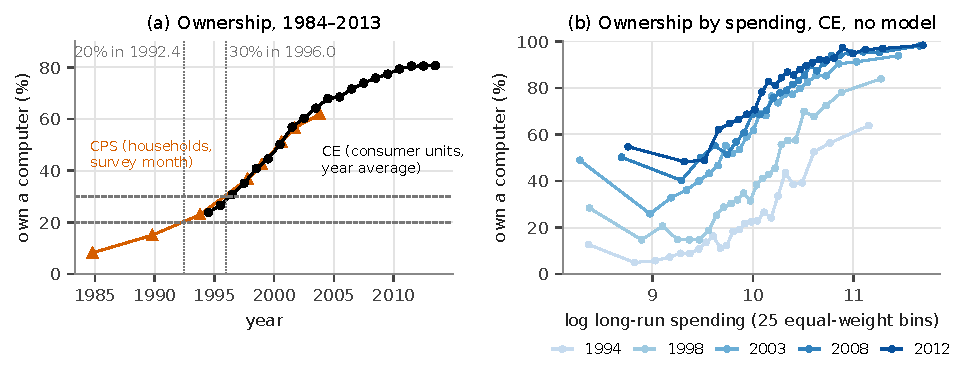
\includegraphics[width=\textwidth]{figures/ownership.pdf}
\caption{Computer ownership, 1984--2013. (a) Share of households that own a computer: CPS households in each of the eight survey months from October 1984 to October 2003, and CE households as a yearly average from 1994 to 2013, with survey weights. Dotted lines mark when the computer ownership rate passed 20\% and 30\% (log-odds interpolation between CPS surveys). (b) Share of CE households that own a computer against log long-run spending, in 25 bins of equal weight, for 1994, 1998, 2003, 2008, and 2012, with no model. A log spending of 10 is \$22{,}000 a year and a log spending of 9 is \$8{,}100.}
\label{fig:own}
\end{figure}

\section{Method}
\label{sec:method}

The method has two stages. The first stage fits a probit model separately for each year from 1994 to 2013, to that year's CE households alone, and estimates the year's spending threshold. The second stage regresses the 20 yearly spending thresholds on the computer price. Estimating a separate model for each year, and only then modelling how the yearly estimates change, lets the data show the path of the spending threshold before we impose any model of that path.

The subscripts run as follows. Years are $t = 1994, \dots, 2013$, which makes 20 years. Households in year $t$ are $i = 1, \dots, N_t$, where $N_t$ is the number of CE households in year $t$: 6{,}153 to 13{,}743 in each year from 1994 to 2012 and 2{,}203 in 2013, so that $N = \sum_t N_t = 178{,}891$ households in all. Geography groups are $g = 1, \dots, 29$. The household-trait vector $z_{it}$ has $K$ entries. $K = 0$ in the baseline regression and with corrected spending alone, $K = 16$ once household traits enter, and $K = 19$ in the extended regression, which adds three education levels of the household head, $e \in \{$less than high school, some college, college degree$\}$, each measured against high school. Table~\ref{tab:steps} lists the regressions. We set the analysis plan before estimation, and Appendix~\ref{app:deviations} lists where we departed from it.

\begin{table}[t]
\centering
\caption{The regressions and the years of data that each uses. The extended regression adds three things to the baseline regression, one at a time, and Appendix~\ref{app:main} reports each intermediate fit.}
\label{tab:steps}
\small
\begin{tabular}{L{0.17\textwidth}L{0.17\textwidth}L{0.58\textwidth}}
\toprule
Regression & Data & What the regression does \\
\midrule
Baseline & CE, 1994--2013 & Estimates a spending threshold for each year from observed long-run spending and the household's state or region, and regresses the 20 yearly spending thresholds on the computer price. \\
\addlinespace
Extended & CE, 1994--2013 & Corrects long-run spending for noise between interviews, then adds household traits (age, the numbers of children and adults, marriage, race, Hispanic origin, and student housing), then adds the education of the household head (the CE's reference person, who owns or rents the home). \\
\addlinespace
CPS extension & CPS, 1984--2003, and CE & Estimates spending thresholds in the CPS, with long-run spending imputed from bracketed income, and tests whether the unexplained trend changed when the computer ownership rate passed 20\% or 30\%. \\
\addlinespace
Robustness checks & CE, 1994--2013 & Fits the extended regression's two stages as one Bayesian model, and repeats the regressions with other samples, spending measures, and price indexes. \\
\bottomrule
\end{tabular}
\end{table}

\subsection{First stage: a spending threshold for each year}
\label{sec:first}

For each year $t$, we fit a probit model, weighted by the CE survey weights, to the year's $N_t$ households. A probit model is a regression model for a yes-or-no outcome, here whether the household owns a computer. The probit model is the empirical form of equation~\eqref{eq:prob}:
\begin{equation}
\Pr(\text{own}_{it} = 1) = \Phi\big(\alpha_t + \beta_t (x_{it} - 10) + \gamma_{g(i),t} + z_{it}'\delta_t\big),
\qquad
\tau_t = 10 - \frac{\alpha_t + \sum_g \pi_g \gamma_{g,t}}{\beta_t},
\end{equation}
where
\begin{itemize}
\item $\text{own}_{it} = 1$ if household $i$, observed in year $t$, has a computer in its appliance inventory;
\item $x_{it}$ is the household's log long-run spending (baseline regression) or its log long-run spending corrected for noise between interviews (extended regression), and subtracting 10 (about \$22{,}000 a year) centres $x_{it}$;
\item $\alpha_t$ is the year's intercept and $\beta_t$ is the year's spending slope;
\item $\gamma_{g,t}$ is the effect of geography group $g$ in year $t$, $g(i)$ is the geography group of household $i$, and $\pi_g$ is group $g$'s pooled 1994--2013 share of households, so that moves of households between places do not shift $\tau_t$;
\item $z_{it}$ is the vector of the household's $K$ traits, centred at their pooled 1994--2013 means, and $\delta_t$ holds the $K$ effects of the traits in year $t$;
\item $\tau_t$ is the spending threshold of a household with the pooled average traits in the pooled average geography, the log long-run spending at which this household's probability of owning a computer is one half.
\end{itemize}

There are 29 geography groups: the 24 states (counting the District of Columbia) that have households in every year and every replicate sample, the rest of each of the four Census regions, and a group for the 1\% of households with no state or region, which is fitted but left out of $\tau_t$. The household traits are the age of the household head (the CE's reference person, the person who owns or rents the home), in seven groups, the numbers of children (none to three or more) and adults (one to three or more), marriage, race (white, black, other), Hispanic origin, and student housing. The extended regression adds the education of the household head in four groups (less than high school, high school, some college, and a college degree), with high school as the reference group. We report an education effect as a shift in the log spending threshold, $\theta_{e,t} = \delta_{e,t}/\beta_t$. A positive $\theta$ means that households with that education own a computer at lower spending than households headed by a high-school graduate.

The extended regression corrects long-run spending for noise between interviews by regression calibration \citep[ch.~4]{carroll2006}, which replaces each household's measured log long-run spending with its expected true value (Appendix~\ref{app:method}). We compute standard errors by balanced repeated replication. We repeat the whole estimation, including the spending correction, with each of the survey's 44 replicate weights, and the variance of an estimate is the mean squared deviation of its replicate estimates from the full-sample estimate.

We use the probit model in every regression. A rule that we set in advance for choosing the link function, the curve that turns household spending into a probability of owning a computer, would switch two of the four CE regressions to a robit model, whose curve is like the probit curve with heavier tails. Appendix~\ref{app:method} describes the rule, and Appendix~\ref{app:deviations} shows that the robit model changes the price effect $b$ little.

\subsection{Second stage: the spending thresholds and the computer price}

We regress the 20 yearly spending thresholds, for $t = 1994, \dots, 2013$, on the computer price in a two-level Bayesian model \citep{lewis2005}, the empirical form of equation~\eqref{eq:path}:
\begin{equation}
\hat\tau_t \sim \text{Normal}(\tau_t, \text{se}_t^2), \qquad
\tau_t = a + b\,\ell_t + d\,(t - 1994) + e_t, \qquad e_t \sim \text{Normal}(0, \omega^2),
\end{equation}
where $\hat\tau_t$ and $\text{se}_t$ are the first-stage spending threshold for year $t$ and its standard error, $a$ is the 1994 spending threshold, $b$ is the price effect, $d$ is the unexplained trend (the yearly change in the log spending threshold), and $e_t$ is year $t$'s deviation from the fitted line beyond sampling error, with standard deviation $\omega$. Pure affordability means $b = 1$ and $d = 0$. The model is hierarchical. Its first level lets each year's estimated spending threshold differ from the year's true spending threshold by sampling error, and its second level relates the 20 true spending thresholds to the computer price, so the second stage has 20 observations. Appendix~\ref{app:method} gives the priors, which are weak, and the sampler settings.

Computer prices vary only by year, so $b$ and $d$ rest on the 20 yearly spending thresholds of 1994--2013, and the 178{,}891 households matter through the precision of those 20 spending thresholds. The second stage can tell $b$ from $d$ only because the computer price fell at different speeds, 27\% a year from 1994 to 2003 and 12\% a year from 2003 to 2012. If the spending threshold fell at the same fraction of the computer price's speed in both periods, that fraction is $b$ and the unexplained trend is zero. If the spending threshold fell at the same speed in both periods, whatever the speed of the computer price, the unexplained trend $d$ accounts for the fall. Even with this variation in the speed of the computer price, the estimates of $b$ and $d$ are tied. Under the main computer price, the posterior correlation of $b$ and $d$ is 0.96 to 0.98 in every specification. A larger $b$ goes with a larger $d$, so the data cannot fully separate a stronger price effect plus an upward unexplained trend from a weaker price effect plus a downward unexplained trend.

\subsection{Splitting the rise between the computer price and household spending}
\label{sec:splitmethod}

We split the 1994--2012 rise in the computer ownership rate between the computer price and household spending by changing one at a time in the household model of the baseline regression. Sections~\ref{sec:split} and~\ref{sec:interaction} use the baseline regression's spending thresholds and spending slopes of 1994--2012, its price effect $b = 0.45$, and each year's observed distribution of household spending (\texttt{income\_price.py}). A household in the pooled average geography owns a computer with probability $\Phi\big(\hat\beta_t(x_{it} - \hat\tau_t)\big)$, and the computer ownership rate is the weighted mean of that probability over the year's households. We start from the 1994 spending threshold and spending slope, and we move the computer price and household spending from their 1994 values to their 2012 values one at a time. We then average the contribution of the computer price, and the contribution of household spending, over the two possible orders of change (a Shapley split). We compute the response of the computer ownership rate to a 10\% cut in the computer price the same way, as the change in each household's predicted probability of owning a computer, averaged over households, which is an average predictive comparison in the sense of \citet{gelman2007apc}. The intervals for these quantities allow for the uncertainty in $b$ only.

\section{Findings}
\label{sec:findings}

From 1994 to 2012 falling quality-adjusted computer prices, far more than rising incomes, paced the spread of home computers (Section~\ref{sec:main}), first among rich households and then among poorer ones (Section~\ref{sec:interaction}), but they left the education gap in computer ownership in place (Section~\ref{sec:educ}). This section reports estimates from the 178{,}891 CE households of 1994--2013 and the main computer price, the BEA price index for personal computers. Throughout, intervals are 90\% intervals in square brackets. For a second-stage coefficient the interval runs from the 5th to the 95th percentile of the posterior distribution, and for a yearly spending threshold it is $\pm 1.645$ replicate standard errors. Dollar amounts are in current dollars unless the text says constant dollars. Appendix~\ref{app:main} gives the estimates in tables, and Section~\ref{sec:robust} summarizes the robustness checks.

\subsection{Falling quality-adjusted computer prices, far more than rising incomes, paced the spread of computers}
\label{sec:main}

Falling prices account for 53 of the 57 percentage points by which the computer ownership rate rose from 1994 to 2012, and rising household spending for 3, even though the median price that households paid for a computer fell only 7\%. The spending threshold followed the quality-adjusted computer price at only about half the strength that pure affordability predicts, but that price fell 98\% from 1994 to 2012, because each dollar bought a better computer.

The spending threshold fell fast in the 1990s, when the computer price fell fast, and slowly after 2003, when the computer price fell slowly, but it fell far less than pure affordability predicts. Figure~\ref{fig:tau} plots the spending threshold in each year from 1994 to 2013, in the baseline regression and as the extended regression adds its three parts, together with the fitted second stage and the path that pure affordability predicts from the 1994 spending threshold. In the baseline regression the spending threshold fell from \$49{,}400 a year in 1994 to \$12{,}700 in 2003 and \$9{,}500 in 2012. From 1994 to 2012 the spending threshold fell by 77--89\% across the four CE regressions, while the quality-adjusted computer price fell by 98\%. In every regression the yearly spending thresholds lie close to the fitted second stage and far above the path that pure affordability predicts.

\begin{figure}[t]
\centering
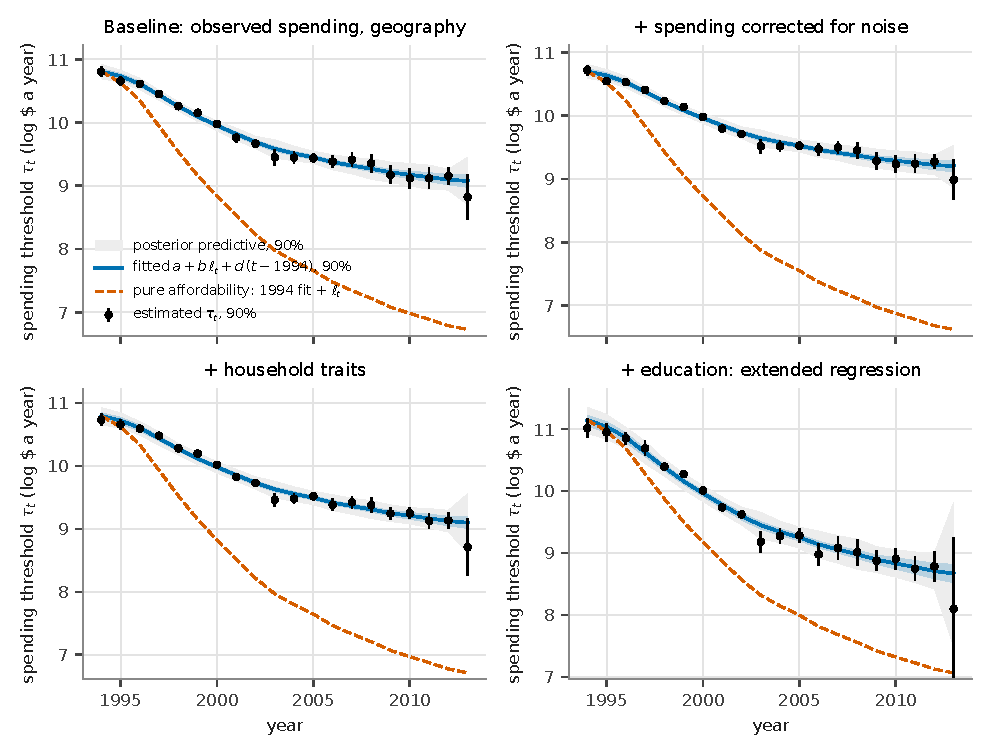
\includegraphics[width=\textwidth]{figures/thresholds.pdf}
\caption{Yearly spending thresholds $\hat\tau_t$, 1994--2013, in the baseline regression and as the extended regression adds its three parts, with 90\% intervals ($\pm 1.645$ replicate standard errors). The spending threshold is the log long-run spending at which a household with average location and traits has a 50\% chance of owning a computer. Blue: the fitted second stage $a + b\,\ell_t + d\,(t - 1994)$ with its 90\% interval. Grey: the 90\% posterior predictive interval, the range in which the fitted second stage expects each year's estimated spending threshold to fall. Dashed: the path that pure affordability predicts, which is the fitted 1994 spending threshold plus $\ell_t$. Main computer price (BEA PCE price index for personal computers). A log spending of 10 is \$22{,}000 a year and a log spending of 9 is \$8{,}100.}
\label{fig:tau}
\end{figure}

\textbf{Across the 20 years from 1994 to 2013, a 10\% fall in the quality-adjusted computer price was associated with a 4--6\% fall in the spending threshold, about half the 10\% fall that pure affordability predicts.} Figure~\ref{fig:effect} puts the second-stage estimates on a percentage scale. In the baseline regression the price effect is $b = 0.45$ $[0.37, 0.54]$, so a 10\% fall in the computer price lowered the spending threshold by 4.6\%. Correcting spending for noise lowers this fall to 4.0\%, and adding household traits leaves it at 4.2\%. Adding the education of the household head raises it to 6.0\% in the extended regression ($b = 0.59$ $[0.46, 0.72]$), and fitting the extended regression as one joint model gives 6.1\%. Every 90\% interval lies below 10\% (Figure~\ref{fig:effect}a).

\textbf{Once the computer price is taken into account, the spending threshold shows no other steady change from 1994 to 2013.} The unexplained trend lies between $-0.5\%$ and $+0.5\%$ a year in all four CE regressions, and the 90\% intervals rule out unexplained trends larger than about 4\% a year in either direction (Figure~\ref{fig:effect}b). Pure affordability predicts an unexplained trend of zero, so an interval that includes zero is the predicted outcome. The spending slope $\beta_t$ shows no trend from 1994 to 2012 either, as prediction 2 requires (Appendix~\ref{app:main}).

\begin{figure}[t]
\centering
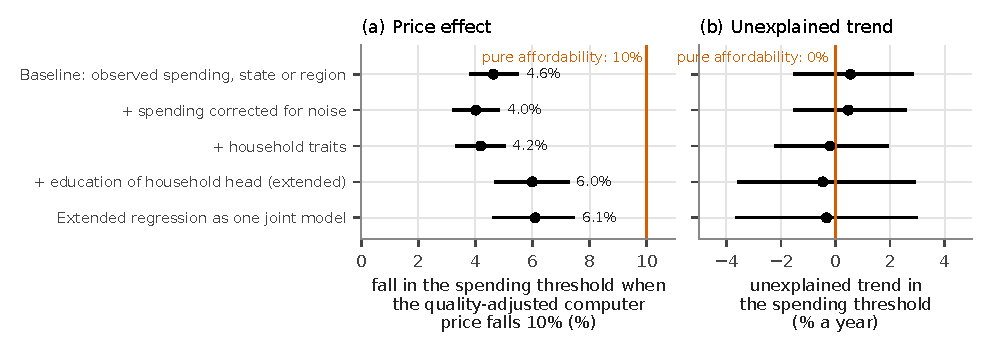
\includegraphics[width=\textwidth]{figures/price_effect.pdf}
\caption{The price effect $b$ and the unexplained trend $d$ on a percentage scale, from the 20 yearly spending thresholds of 1994--2013, main computer price: posterior medians with 90\% intervals. (a) The fall in the spending threshold when the quality-adjusted computer price falls 10\%, $100\,(1 - 0.9^{b})$ percent. Pure affordability ($b = 1$) predicts a fall of 10\%. (b) The unexplained trend, the yearly change in the spending threshold that the computer price does not explain, $100\,(e^{d} - 1)$ percent a year. Pure affordability predicts 0\%. The first four rows are the two-stage fits of Section~\ref{sec:method}, from the baseline regression to the extended regression, and the last row fits the extended regression as one joint model of all 178{,}891 CE households (Appendix~\ref{sec:joint}).}
\label{fig:effect}
\end{figure}

Because the price effect is about one half, pure affordability predicts a much faster spread of computers from 1994 to 2012 than occurred. Applied to 2012 households at the 2012 computer price, the 1994 probit model predicts that nearly every household owned a computer by 2012, against the actual 81\% (Appendix~\ref{app:pure}).

\label{sec:split}
\textbf{Even at half strength, falling prices raised computer ownership far more than rising incomes did.} Falling computer prices alone would have raised the computer ownership rate from 24\% in 1994 to 77\% in 2012, close to the actual 81\%, while rising household spending alone would have raised it only to 27\%. Figure~\ref{fig:paths} shows what the computer ownership rate would have been in each year from 1994 to 2012 if only one of the two forces had changed after 1994, according to the baseline regression. Both forces are measured in constant 1994 dollars. In the blue path, the quality-adjusted computer price falls as it did, and household spending keeps its 1994 distribution. In the orange path, household spending rises as it did after inflation, and the computer price stays at its 1994 level relative to all consumer prices. With both forces at work, the model's path (dashed) stays within 2.6 percentage points of the actual computer ownership rate in every year from 1994 to 2012.

\begin{figure}[t]
\centering
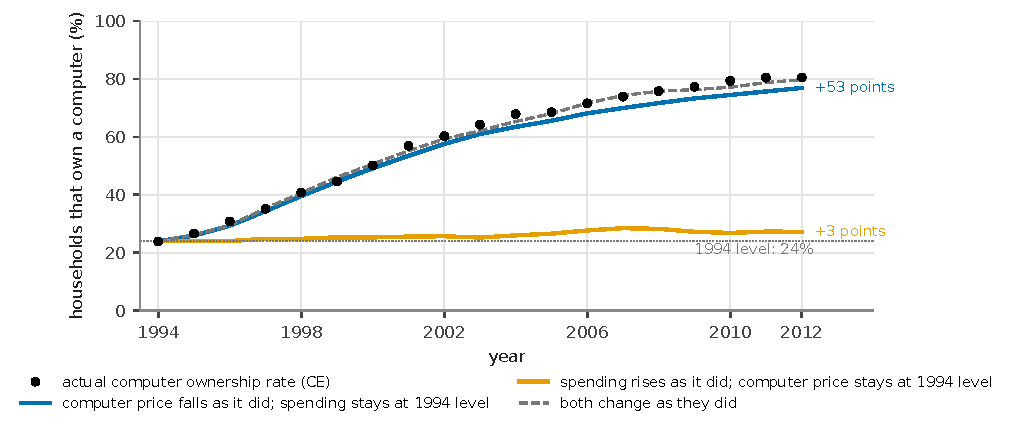
\includegraphics[width=\textwidth]{figures/paths.pdf}
\caption{The computer ownership rate of US households, 1994--2012, if only the computer price or only household spending had changed after 1994 (baseline regression, price effect $b = 0.45$, constant 1994 dollars). Blue: the quality-adjusted computer price, relative to all consumer prices, falls as it did, and household spending keeps its 1994 distribution. Orange: household spending rises as it did after inflation, and the computer price stays at its 1994 level relative to all consumer prices. Dashed: both change as they did. Dots: the actual computer ownership rate of CE households, with survey weights. Every path starts from the 1994 spending threshold and spending slope (Section~\ref{sec:splitmethod}).}
\label{fig:paths}
\end{figure}

The computer price did most of the work because it changed far more than household spending did. From 1994 to 2012 the quality-adjusted computer price, relative to all consumer prices, fell to 1/79 of its 1994 level. Over the same years the long-run spending of the median household rose by 14\% after inflation, from \$19{,}200 to \$21{,}900 a year in 1994 dollars. Because the price effect is about one half, a 1\% rise in household spending did about as much for computer ownership as a 2\% fall in the computer price, but the computer price fell much further than household spending rose.

\textbf{The fall in the computer price accounts for 52.8 percentage points of the 1994--2012 rise in the computer ownership rate, or 94\% of the part that prices and incomes explain (93\% to 96\% across the 90\% interval for $b$), and the growth of household spending accounts for 3.1 points, or 6\%.} These shares average over the two orders in which the two changes can be made (a Shapley split, Section~\ref{sec:splitmethod}). A split in current dollars counts general inflation as growth in household spending, and that split gives household spending 19\% of the part of the 1994--2012 rise that prices and incomes explain (Appendix~\ref{app:main}).

\label{sec:quality}
\textbf{Quality improvement, more than lower dollar prices, paced the spread of computers.} Most of the fall in the quality-adjusted computer price from 1994 to 2012 came from better computers, and little of it from lower dollar prices. Figure~\ref{fig:prices} plots each computer price, monthly, relative to its 1994 average. From 1994 to 2012 the quality-adjusted computer price fell to 1/56 of its 1994 level (by 4.02 in logs). From 1994 to 2012 the dollar price that CE households paid for a computer fell by only 7\% at the median and by 47\% at the 90th percentile. The dollar price of a computer equals its quality-adjusted price times its quality, so the fall in the quality-adjusted price splits into a rise in quality and a fall in the dollar price. Measured in logs, better computers account for 84--98\% of the 1994--2012 fall in the quality-adjusted computer price, and lower dollar prices account for the rest. The dollar price fell far less than the quality-adjusted price because the gains in technology went into better computers and into productization, the work of turning the computer into a product that ordinary households could buy and use. The median price paid is a noisy series that rose after 2010, which may partly reflect the CE's move of computer accessories to a code of their own in the second quarter of 2011. The 90th percentile is steadier, so the lower bound of 84\% is the firmer number.

\begin{figure}[t]
\centering
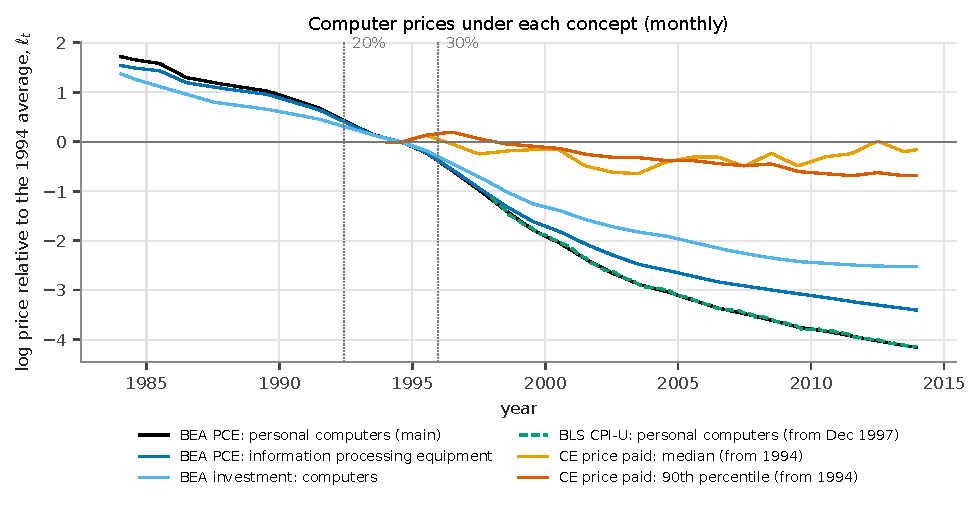
\includegraphics[width=\textwidth]{figures/prices.pdf}
\caption{Log computer price under each price concept, monthly from 1984 to 2013, relative to the 1994 average. A fall of 1 in the log price is a fall to 37\% of the earlier price, and a fall of 4 is a fall to 1.8\%. The BLS consumer price index for all urban consumers (CPI-U) for personal computers starts in December 1997 and is anchored to the main index's 1999 level. The price paid is the CE's weighted median and 90th percentile of reported purchase prices for computers.}
\label{fig:prices}
\end{figure}

\textbf{The other quality-adjusted computer price indexes give similar price effects, but the dollar price that households paid explains almost none of the fall in the spending threshold.} The two other BEA price indexes give price effects between 0.39 and 0.79 over 1994--2013, and the CPI-U for personal computers, which covers only 1999--2013, gives 0.63 to 0.93 (Appendix~\ref{app:prices}). Measured against the median price paid, the computer price explains almost none of the 77--89\% fall in the spending threshold from 1994 to 2012, and an unexplained trend of 8--12\% a year accounts for nearly all of that fall (Appendix~\ref{app:main}).

\subsection{As computer prices fell, the gap in computer ownership between rich and poor households widened, then narrowed}
\label{sec:interaction}

\textbf{The gap between the computer ownership rates of the richest and poorest fifths of households widened from 39.3 percentage points in 1994 to 53.8 in 2003, and then narrowed to 36.6 in 2012, slightly below its 1994 level} (Figure~\ref{fig:fifths}b). Figure~\ref{fig:fifths}a shows the computer ownership rate in each fifth of reported household income, in each year from 1994 to 2013 except 2004 and 2005, whose CE files carry no income ranking. From 1994 to 2003 the computer ownership rate of the richest fifth rose by 41 percentage points, from 49.8\% to 91.2\%, and the computer ownership rate of the poorest fifth rose by 27 points, from 10.5\% to 37.4\%. From 2003 to 2012 the richest fifth gained 6 points, to 96.9\%, and the poorest fifth gained 23 points, to 60.3\%. The gains in computer ownership moved down the income distribution, as the spending threshold did.

\begin{figure}[t]
\centering
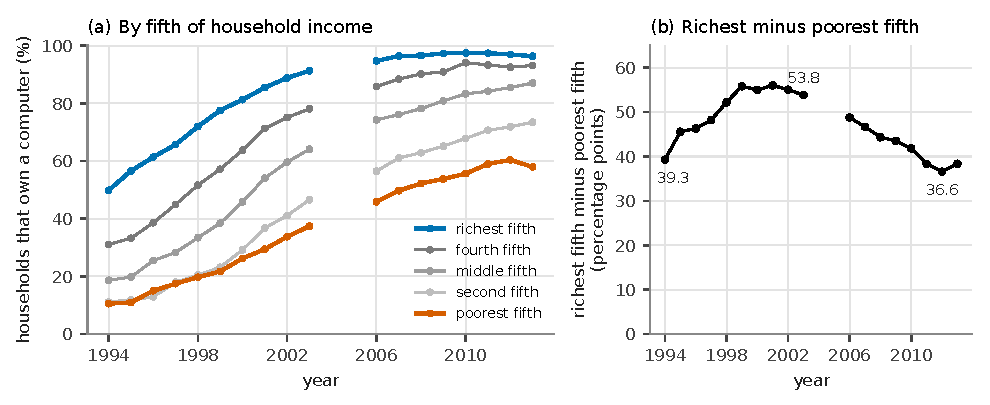
\includegraphics[width=\textwidth]{figures/fifths.pdf}
\caption{Computer ownership by fifth of household income, CE, 1994--2013, with survey weights. (a) The share of households that own a computer in each fifth of reported income, among CE interviews with the appliance inventory and a complete income report, with households ranked by the CE's own income ranking. The CE files for 2004 and 2005 carry no income ranking. (b) The computer ownership rate of the richest fifth minus the computer ownership rate of the poorest fifth, in percentage points.}
\label{fig:fifths}
\end{figure}

The gap widened from 1994 to 2003 and narrowed from 2003 to 2012 because, over those years, the spending threshold fell from the top of the distribution of household spending to the bottom. Figure~\ref{fig:interaction}a places each year's spending threshold in that year's distribution of long-run spending. In 1994, 95\% of households spent less than the spending threshold, so only the top 5\% of households were more likely than not to own a computer. The spending threshold passed the spending of the median household between 1999 and 2000, as the computer ownership rate passed 50\%. By 2012 only 4\% of households spent less than the spending threshold.

\textbf{Every household faced the same computer price, but from 1994 to 2012 the households that a price cut helped most moved from the top of the income distribution to the bottom.} Figure~\ref{fig:interaction}b shows how much a 10\% fall in the quality-adjusted computer price raised a household's probability of owning a computer, by the household's percentile of long-run spending. In 1994 the rise was largest near the top of the spending distribution, 1.55 percentage points at the 90th percentile against 0.55 at the 10th percentile. In 2012 the rise was largest near the bottom, 1.51 points at the 10th percentile against 0.39 at the 90th percentile. In the 1990s, when price cuts mostly helped high-income households, the gap in computer ownership between rich and poor households widened. After 2003, when most high-income households already owned a computer and price cuts mostly helped low-income households, the gap narrowed.

A 10\% cut in the computer price brought in the most new computer owners in 1999 and 2000, when the spending threshold stood near the spending of the median household and the most households had spending near the spending threshold. Figure~\ref{fig:interaction}c averages over households. The 10\% cut raised the computer ownership rate by 1.10 percentage points $[0.89, 1.32]$ in 1994, by 1.37 points in 1999 and 2000, and by 0.94 points $[0.77, 1.12]$ in 2012. From 2000 on the spending threshold lay in the bottom half of the spending distribution, so the number of new computer owners that each price cut brought in depended on the incomes of the bottom half of households.

\begin{figure}[t]
\centering
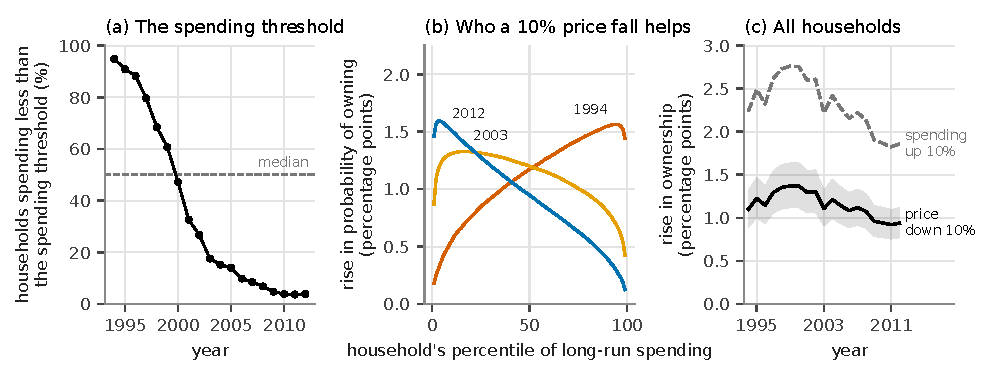
\includegraphics[width=\textwidth]{figures/income_price.pdf}
\caption{Household spending, the computer price, and their interaction (baseline regression, main computer price, $b = 0.45$). (a) Share of households whose long-run spending is below the spending threshold $\hat\tau_t$, in each year from 1994 to 2012, the log long-run spending at which a household with average location and traits has a 50\% chance of owning a computer. (b) Rise in a household's probability of owning a computer from a 10\% fall in the quality-adjusted computer price, $\Phi\big(\hat\beta_t(x - \hat\tau_t + b \ln(1/0.9))\big) - \Phi\big(\hat\beta_t(x - \hat\tau_t)\big)$, by the household's percentile of long-run spending, for a household in the pooled average geography, in 1994, 2003, and 2012. (c) The same rise averaged over households in each year from 1994 to 2012, with a 90\% band from $b$ alone, and the rise from a 10\% rise in every household's spending.}
\label{fig:interaction}
\end{figure}

\subsection{Falling computer prices still left the education gap in computer ownership in place}
\label{sec:educ}

In the CE data, with survey weights and no model, the gap in computer ownership between households headed by college graduates and households headed by high-school graduates widened as computer prices fell in the 1990s and narrowed only after 2001. The gap between the two groups' computer ownership rates was 29.8 percentage points in 1994 and 39.3 in 1997, stayed above 36 points through 2001, and then fell to 22.9 in 2012. As with the gap between rich and poor households, the education gap narrowed only once most households in the leading group already owned a computer, which for college households was from 2001 on, when more than 80\% of them did. The gap between college households and households whose head did not finish high school grew from 38.0 points in 1994 to 59.4 in 2001 and was still 43.8 in 2012.

\textbf{Among households with the same long-run spending, the education gap did not shrink as the computer price fell.} Figure~\ref{fig:educ} shows, for each year from 1994 to 2012, the spending threshold of households in each education group of the extended regression, relative to the spending threshold of otherwise similar households headed by a high-school graduate. Averaged over 1994--2012, the spending threshold of households headed by a college graduate was about one third (0.35) of the spending threshold of households headed by a high-school graduate. \textbf{A household headed by a college graduate that spent \$10{,}000 a year was as likely to own a computer as an otherwise similar household headed by a high-school graduate that spent \$28{,}000, or 2.8 times as much.} The multiple was 2.4 in 1994 and again in 2012, and a weighted linear trend puts its change at $+0.2\%$ a year $[-0.9\%, +1.3\%]$. The college ratio lies between 0.32 and 0.45 in every year except 2003 and 2006 (0.21 and 0.24), the two years with the flattest spending slope. Averaged over 1994--2012, households headed by someone with some college had about half the spending threshold of high-school households (0.51), and households headed by someone who did not finish high school had 1.67 times the spending threshold of high-school households, and these gaps did not shrink either. \emph{Prediction 3 fails.} At the same long-run spending, more educated households owned computers earlier.

\begin{figure}[t]
\centering
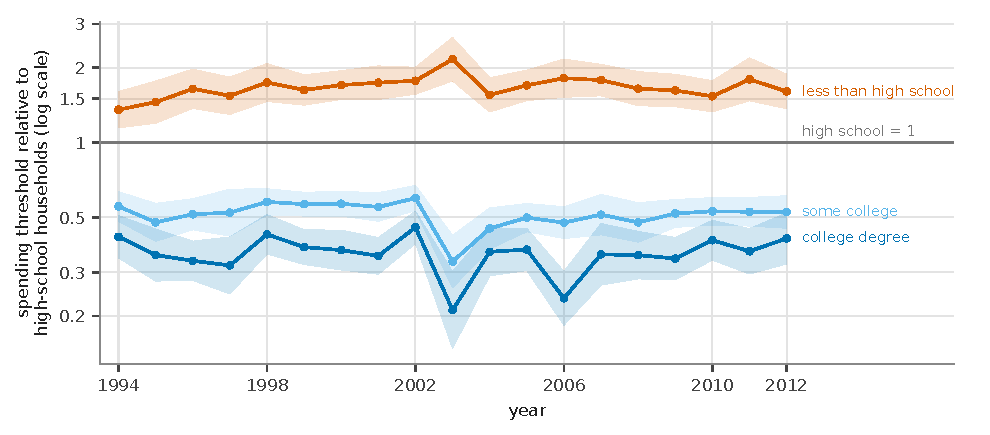
\includegraphics[width=\textwidth]{figures/education.pdf}
\caption{Spending thresholds by education of the household head, extended regression, 1994--2012, relative to the spending threshold of otherwise similar households headed by a high-school graduate, with 90\% intervals ($\pm 1.645$ replicate standard errors), on a log scale. Each line is $\exp(-\theta_{e,t})$ for education level $e$ in year $t$. A value of 0.35 means that a household with that education was as likely to own a computer as a household headed by a high-school graduate that spent $1/0.35 = 2.8$ times as much. The education shift is $\theta_{e,t} = \delta_{e,t}/\beta_t$ (Section~\ref{sec:first}), so in 2003 and 2006, the two years with the flattest spending slope $\beta_t$, every education shift is larger.}
\label{fig:educ}
\end{figure}

The college gap could partly reflect income that long-run spending misses. A control function, which uses current income as an instrument for long-run spending (Appendix~\ref{sec:checks}), shrinks the college shift, averaged over 1994--2012, by about a quarter. With the control function, a household headed by a college graduate was still as likely to own a computer as a household headed by a high-school graduate that spent 2.2 times as much (Appendix~\ref{app:main}).

\subsection{Robustness}
\label{sec:robust}

The estimates hold up in the robustness checks of Appendix~\ref{app:results}. Fitting the extended regression's two stages at once, as one Bayesian model of all 178{,}891 CE households of 1994--2013, gives $b = 0.60$ $[0.45, 0.74]$ and $d = -0.003$ $[-0.038, 0.029]$, against 0.59 and $-0.005$ from the two stages. Under most other choices of sample, spending measure, and link function, $b$ stays between 0.37 and 0.61, and in constant dollars $b$ is within 0.02 of its current-dollar value. Two checks give larger price effects. Counting vehicle purchases as spending gives 0.88 $[0.71, 1.05]$ in the extended regression, and replacing long-run spending with current income, a measure of long-run resources with much noise, gives 1.38 $[0.86, 1.95]$. Apart from current income, $d$ stays between $-0.014$ and $+0.031$ a year. The second-stage model fits the yearly spending thresholds, and the two-stage method recovers known values of $b$ and $d$ from fake data.

\section{Discussion}
\label{sec:discussion}

\paragraph{What the results say about the profit switch.} \textbf{The results support the affordability phase of the profit switch hypothesis in part.} From 1994, when 24\% of US households owned a computer, to 2012, the spending threshold moved in step with the quality-adjusted computer price and showed no other steady change, so affordability matches the timing of the spread of computers over those years. But the spending threshold fell only about half as fast as the computer price, in percentage terms, and education shifted the spending threshold at a given level of spending, so affordability alone does not account for which households owned a computer. The first phase of the hypothesis, in which firms' profits and investment pace the spread of a technology, lies before spring 1992, when the computer ownership rate passed 20\%, and only two surveys, the CPS supplements of October 1984 and October 1989, measure computer ownership in those years. The surveys therefore cannot test whether the forces behind computer ownership switched between the two phases. When we fit the CPS and CE spending thresholds together, the unexplained trend appears to change in late 1995, when the computer ownership rate passed 30\%, but that change falls where the data move from the CPS to the CE, and within the CPS alone a model with one unexplained trend predicts best (Appendix~\ref{sec:cps}).

\paragraph{Why the price effect is about one half.} The household model offers two readings of a price effect of about 0.5. In the first reading, other costs of owning a computer, such as software, an internet connection, and the time it takes to learn to use a computer, fell more slowly than the hardware price and made up about half of the cost of ownership. In the second reading, households valued only part of the quality improvement that the price index counts. A faster processor counts fully in the price index but may matter little to a household that uses its computer for email and letters. \emph{Both readings say that the effective cost of owning a computer fell about half as fast, in percentage terms, as the quality-adjusted computer price.} Our data cannot tell the two readings apart. The size of the price effect also depends on which quality-adjusted index is used, and the BEA indexes that fell less than the main index give price effects of up to 0.79 over 1994--2013 (Appendix~\ref{app:prices}). Measures based on computing performance show larger price falls than the official indexes \citep{nordhaus2007}, and against such measures the price effect would be smaller still.

\paragraph{What the absence of an unexplained trend means.} An unexplained trend near zero means that, nationally, nothing other than the computer price changed the spending threshold steadily from 1994 to 2013. Spillovers from learning or from networks that grew steadily with computer ownership would have made the spending threshold fall faster than the computer price explains, which would show up as a negative unexplained trend. The estimates rule out unexplained trends larger than about 4\% a year, and the fake-data check of Appendix~\ref{sec:checks} shows that an unexplained trend of about 5\% a year would have been detected. Smaller unexplained trends remain possible, and because the estimates of $b$ and $d$ are tied, a negative unexplained trend would come with an even smaller price effect. Local spillovers of the kind that \citet{goolsbee2002} find need not show up as a national trend.

\paragraph{What the education gap means.} Among households with the same long-run spending, the education gap in computer ownership was large from 1994 to 2012 and did not shrink as computer prices fell, even though the raw gap narrowed after 2001 as most college households came to own a computer. Part of the education gap may be income that long-run spending misses, since the control function shrinks the gap by about a quarter. The rest of the gap suggests that, at the same resources, more educated households valued a computer more, found a computer easier to use, or knew more about computers. Our data cannot separate those readings.

\paragraph{How the findings compare with earlier work.} Our findings fit the closest earlier work, and they add what falling computer prices changed and what they left in place. \citet{chinn2007} find that differences in income per head account for most of the gap in computer and internet use across 161 countries in 1999--2001. We find that falling prices account for 94\% of the 1994--2012 rise in US computer ownership that prices and incomes explain. The two findings need not conflict. \citet{chinn2007} compare countries at one point in time, when incomes differ widely across countries, while we follow one country over the 18 years from 1994 to 2012, in which the quality-adjusted computer price fell to 1/56 of its 1994 level and the long-run spending of the median household rose by 14\% after inflation. The order in which income groups bought computers matches the finding of \citet[p.~111]{greenwood2005} that poor households bought durable goods later than rich households, when prices were lower. Our household model adds why the gap between rich and poor households widened from 1994 to 2003. A price cut does the most for households close to buying, and in 1994 the households close to buying a computer were the richest households. The education gap in computer ownership matches evidence on computer use at work \citep{riddell2017} and on generative AI. \citet{bick2024} find that generative AI and the personal computer had similar early adoption patterns by education (Section~\ref{sec:ai}). We add that, at the same long-run spending, the education gap in home computer ownership did not shrink from 1994 to 2012, while the quality-adjusted computer price fell 98\%.

\paragraph{Limits.} Computer prices are the same for every household in a given year, so the price effect and the unexplained trend rest on the 20 yearly spending thresholds of 1994--2013. The estimates of the price effect and the unexplained trend therefore also pick up anything else that moved with computer prices over time, including the spread of the internet and of software, and network effects among computer users \citep{goolsbee2002}. The household data can measure an unexplained trend, but the household data cannot say what caused an unexplained trend. The early phase of the spread of computers is thinly observed, since only the CPS supplements of October 1984 and October 1989 measure computer ownership while the computer ownership rate was below 20\%, and those two supplements record current income in brackets. The CE computer ownership question changed its wording in the second quarter of 2001, and the CPS education question changed between 1989 and 1993, mainly between high school and some college \citep{jaeger1997}. We estimate the mapping from income to spending in 1994--1998 and apply the mapping to every CPS year, and the 2013 spending thresholds rest on one quarter of data.

\section{Implications for AI diffusion and policy}
\label{sec:ai}

Generative AI has spread faster than the personal computer did. Figure~\ref{fig:ai}a counts years from the first mass-market product of each technology, the IBM PC in August 1981 and ChatGPT in November 2022, the dates that \citet{bick2024} use. In August 2025, less than three years after the release of ChatGPT, 54.6\% of US adults aged 18 to 64 used generative AI, up from 44.6\% in August 2024 \citep{bick2025state}. In 1984, three years after the IBM PC went on sale, 19.7\% of US adults aged 18 to 64 used a personal computer \citep{bick2025state}, and 8.2\% of US households owned a computer. The share of US households that owned a computer passed 50\% only in 2000, nineteen years after the IBM PC went on sale.

\begin{figure}[t]
\centering
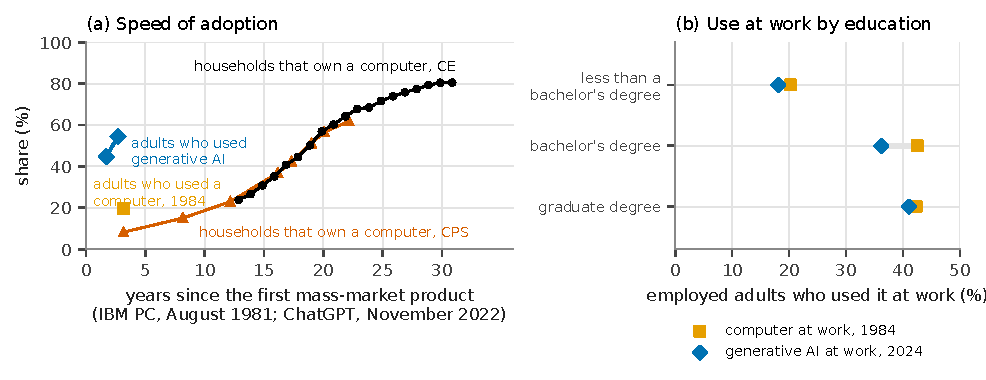
\includegraphics[width=\textwidth]{figures/ai_pc.pdf}
\caption{Home computers and generative AI in the United States. (a) Adoption by years since each technology's first mass-market product, the IBM PC (August 1981) and ChatGPT (November 2022). Black and red: the share of households that own a computer, from the CE (yearly averages, 1994--2012) and the CPS supplements (October 1984 to October 2003). Orange: the share of adults aged 18 to 64 who used a personal computer in 1984. Blue: the share of adults aged 18 to 64 who used generative AI in August 2024 and August 2025, from the Real-Time Population Survey (RPS) of \citet{bick2024}. The orange and blue points are published estimates \citep{bick2025state}. (b) The share of employed adults aged 18 to 64 who used a computer at work in October 1984 (CPS) and who used generative AI at work in August and November 2024 (RPS), by education \citep[Figure 5a]{bick2024}.}
\label{fig:ai}
\end{figure}

As with the computer, more educated adults adopted generative AI first (Figure~\ref{fig:ai}b). In October 1984, 42.5\% of employed adults aged 18 to 64 with a bachelor's degree used a computer at work, against 20.2\% of employed adults without a bachelor's degree. In August and November 2024, 36.2\% of employed adults with a bachelor's degree used generative AI at work, against 18.1\% of employed adults without a bachelor's degree \citep[Figure 5a]{bick2024}. For both technologies, workers with a bachelor's degree were about twice as likely as workers without one to use the technology at work.

Much of the use of generative AI costs households nothing in dollars. \citet{bick2024} point to low adoption costs as one likely reason that generative AI spread faster than the personal computer outside work, since a computer required expensive hardware while generative AI is available free or with a low-cost subscription. The basic tiers of the main AI assistants are free, and the paid tiers are subscriptions at fixed dollar prices. Anthropic's Claude Pro subscription, for example, cost \$20 a month when it launched in September 2023 \citep{anthropic2023}, and Claude Pro still cost \$20 a month in November 2026 \citep{anthropic2026}. The adoption rates in Figure~\ref{fig:ai} count any use of generative AI, paid or free.

Firms can also gain from AI use indirectly, through advertising and through users' data. OpenAI said in January 2026 that it would test advertising in the United States in the free tier of ChatGPT and in its low-cost Go plan, while keeping its higher-priced plans free of ads \citep{openai2026}, and since 2025 Anthropic has asked users of its free and paid consumer plans whether their conversations may be used to train its models \citep{anthropic2025}. In the terms of the profit switch hypothesis, free tiers are one way that firms' profits and investment pace the early adoption of AI, and advertising and data may let firms keep AI free to many households long after the early phase. How far AI funded in these ways spreads may then depend more on what firms earn from it than on what households can spend. The household model of this paper compares what a household can spend with a dollar price, so the implications below hold only for AI that households pay for in dollars, such as subscriptions.

If paid AI services follow the pattern that home computers followed after 1994, when 24\% of US households owned a computer, \textbf{the spread of paid AI may follow affordability measured against a quality-adjusted price of AI services}. Paid consumer AI has mostly been sold at fixed monthly prices while the capability of AI rose. From 1994 to 2012 the dollar price that households paid for computers fell far less than the quality-adjusted computer price, which fell to 1/56 of its 1994 level, and measured against the dollar price, affordability explains almost none of the spread of computers. The subscription price of AI may say as little about the spread of paid AI. If the price effect estimated for computers over 1994--2013 carries over to AI, \textbf{a 10\% fall in the quality-adjusted price of AI services would lower the spending threshold for paid AI by 4--6\%}, and a 1\% rise in household spending would do as much for paid AI adoption as a fall of about 2\% in that price. For computers, the quality-adjusted price fell so far from 1994 to 2012 that falling prices account for 94\% of the rise in computer ownership over those years that prices and incomes together explain, so if the quality-adjusted price of AI services falls as fast, income growth would set little of the pace of paid AI adoption.

Every household would face the same price for a paid AI service, but \textbf{a fall in that price would be most likely to tip households close to paying for AI into paying for it}, the households whose spending is near the spending threshold for paid AI. At first these would be high-income households, and as the spending threshold falls they would be lower-income households, so the gap in paid AI use between rich and poor households may first widen and then narrow, as the gap in computer ownership did. \textbf{Once the spending threshold for paid AI falls below the spending of the median household, how many households each price cut brings to paid AI would depend on the incomes of the bottom half of households.} This prediction offers a household mechanism for the companion cross-country finding that, above a switch point of about 5\% of the population, internet adoption rose faster in countries with a larger bottom-50\% income share (an association across 22 advanced economies, 1991--2016). Cheaper AI may do less for the education gap. For computers, averaged over 1994--2012, a household headed by a college graduate was as likely to own a computer as an otherwise similar household headed by a high-school graduate that spent 2.8 times as much, and this gap did not close as computer prices fell, so \textbf{falling prices may leave gaps in paid AI adoption between more and less educated households with the same income in place}.

For policy, the first need is measurement. \textbf{Policymakers will need a quality-adjusted price index for AI services, of the kind that the BEA and BLS publish for computers, to track how affordable AI is becoming.} Testing the profit switch hypothesis or its affordability phase for AI also requires a household survey that records AI use, paid or free, together with income or spending from early adoption on, ideally every year. The CPS computer supplements began in 1984, when 8\% of households owned a computer, but ran only every four or five years before 1997. With both kinds of data, the two stages of this paper can be run below and above 20--30\% adoption, and the price effect and the unexplained trend can be compared across the switch.

\textbf{Once the spending threshold for paid AI is below the spending of the median household, a given amount of income support or price subsidy would raise paid AI adoption more if it went to the bottom half of households than if it were spread across all households}, because the households close to adopting would then be lower-income households. Cheaper AI alone may leave the education gap in place.

\begingroup\raggedright
\begin{thebibliography}{99}
\bibitem[Anthropic(2023)]{anthropic2023} Anthropic (2023). Introducing Claude Pro. 7 September 2023. \url{https://www.anthropic.com/news/claude-pro}.
\bibitem[Anthropic(2025)]{anthropic2025} Anthropic (2025). Updates to consumer terms and privacy policy. 28 August 2025. \url{https://www.anthropic.com/news/updates-to-our-consumer-terms}.
\bibitem[Anthropic(2026)]{anthropic2026} Anthropic (2026). Claude plans and pricing. Accessed 11 November 2026. \url{https://www.claude.com/pricing}.
\bibitem[Berndt and Rappaport(2001)]{berndt2001} Berndt, E. R., and N. J. Rappaport (2001). Price and quality of desktop and mobile personal computers: A quarter-century historical overview. \emph{American Economic Review} 91(2), 268--273. \href{https://doi.org/10.1257/aer.91.2.268}{doi:10.1257/aer.91.2.268}.
\bibitem[Bick et~al.(2024)Bick, Blandin, and Deming]{bick2024} Bick, A., A. Blandin, and D. J. Deming (2024). The rapid adoption of generative AI. NBER Working Paper 32966, revised February 2025. \href{https://doi.org/10.3386/w32966}{doi:10.3386/w32966}. Published in \emph{Management Science} 72(10), 8440--8456 (2026), \href{https://doi.org/10.1287/mnsc.2025.02523}{doi:10.1287/mnsc.2025.02523}.
\bibitem[Bick et~al.(2025)Bick, Blandin, and Deming]{bick2025state} Bick, A., A. Blandin, and D. J. Deming (2025). The state of generative AI adoption in 2025. Federal Reserve Bank of St. Louis, \emph{On the Economy}, 13 November 2025. \url{https://www.stlouisfed.org/on-the-economy/2025/nov/state-generative-ai-adoption-2025}.
\bibitem[Blundell et~al.(2008)Blundell, Pistaferri, and Preston]{blundell2008} Blundell, R., L. Pistaferri, and I. Preston (2008). Consumption inequality and partial insurance. \emph{American Economic Review} 98(5), 1887--1921. \href{https://doi.org/10.1257/aer.98.5.1887}{doi:10.1257/aer.98.5.1887}.
\bibitem[Bonus(1973)]{bonus1973} Bonus, H. (1973). Quasi-Engel curves, diffusion, and the ownership of major consumer durables. \emph{Journal of Political Economy} 81(3), 655--677. \href{https://doi.org/10.1086/260063}{doi:10.1086/260063}.
\bibitem[Bowling et~al.(2009)Bowling, Khasawneh, Kaewkuekool, and Cho]{bowling2009} Bowling, S. R., M. T. Khasawneh, S. Kaewkuekool, and B. R. Cho (2009). A logistic approximation to the cumulative normal distribution. \emph{Journal of Industrial Engineering and Management} 2(1), 114--127. \href{https://doi.org/10.3926/jiem.2009.v2n1.p114-127}{doi:10.3926/jiem.2009.v2n1.p114-127}.
\bibitem[B{\"u}rkner(2017)]{burkner2017} B{\"u}rkner, P.-C. (2017). brms: An R package for Bayesian multilevel models using Stan. \emph{Journal of Statistical Software} 80(1), 1--28. \href{https://doi.org/10.18637/jss.v080.i01}{doi:10.18637/jss.v080.i01}.
\bibitem[Carpenter et~al.(2017)]{carpenter2017} Carpenter, B., A. Gelman, M. D. Hoffman, D. Lee, B. Goodrich, M. Betancourt, M. Brubaker, J. Guo, P. Li, and A. Riddell (2017). Stan: A probabilistic programming language. \emph{Journal of Statistical Software} 76(1), 1--32. \href{https://doi.org/10.18637/jss.v076.i01}{doi:10.18637/jss.v076.i01}.
\bibitem[Carroll et~al.(2006)Carroll, Ruppert, Stefanski, and Crainiceanu]{carroll2006} Carroll, R. J., D. Ruppert, L. A. Stefanski, and C. M. Crainiceanu (2006). \emph{Measurement Error in Nonlinear Models: A Modern Perspective}, 2nd ed. Boca Raton: Chapman and Hall/CRC. \href{https://doi.org/10.1201/9781420010138}{doi:10.1201/9781420010138}.
\bibitem[Chinn and Fairlie(2007)]{chinn2007} Chinn, M. D., and R. W. Fairlie (2007). The determinants of the global digital divide: A cross-country analysis of computer and internet penetration. \emph{Oxford Economic Papers} 59(1), 16--44. \href{https://doi.org/10.1093/oep/gpl024}{doi:10.1093/oep/gpl024}.
\bibitem[David(1969)]{david1969} David, P. A. (1969). A contribution to the theory of diffusion. Research Center in Economic Growth, Memorandum 71, Stanford University.
\bibitem[Fairlie(2005)]{fairlie2005} Fairlie, R. W. (2005). An extension of the Blinder-Oaxaca decomposition technique to logit and probit models. \emph{Journal of Economic and Social Measurement} 30(4), 305--316. \href{https://doi.org/10.3233/JEM-2005-0259}{doi:10.3233/JEM-2005-0259}.
\bibitem[Friedman(1957)]{friedman1957} Friedman, M. (1957). \emph{A Theory of the Consumption Function}. Princeton: Princeton University Press.
\bibitem[Gelman and Hill(2007)]{gelman2007} Gelman, A., and J. Hill (2007). \emph{Data Analysis Using Regression and Multilevel/Hierarchical Models}. Cambridge: Cambridge University Press. \href{https://doi.org/10.1017/CBO9780511790942}{doi:10.1017/CBO9780511790942}.
\bibitem[Gelman and Pardoe(2007)]{gelman2007apc} Gelman, A., and I. Pardoe (2007). Average predictive comparisons for models with nonlinearity, interactions, and variance components. \emph{Sociological Methodology} 37(1), 23--51. \href{https://doi.org/10.1111/j.1467-9531.2007.00181.x}{doi:10.1111/j.1467-9531.2007.00181.x}.
\bibitem[Gelman et~al.(2020)]{gelman2020} Gelman, A., A. Vehtari, D. Simpson, C. C. Margossian, B. Carpenter, Y. Yao, L. Kennedy, J. Gabry, P.-C. B{\"u}rkner, and M. Modr{\'a}k (2020). Bayesian workflow. arXiv:2011.01808. \url{https://arxiv.org/abs/2011.01808}.
\bibitem[Geroski(2000)]{geroski2000} Geroski, P. A. (2000). Models of technology diffusion. \emph{Research Policy} 29(4--5), 603--625. \href{https://doi.org/10.1016/S0048-7333(99)00092-X}{doi:10.1016/S0048-7333(99)00092-X}.
\bibitem[Goolsbee and Klenow(2002)]{goolsbee2002} Goolsbee, A., and P. J. Klenow (2002). Evidence on learning and network externalities in the diffusion of home computers. \emph{Journal of Law and Economics} 45(2), 317--343. \href{https://doi.org/10.1086/344399}{doi:10.1086/344399}.
\bibitem[Greenwood et~al.(2005)Greenwood, Seshadri, and Yorukoglu]{greenwood2005} Greenwood, J., A. Seshadri, and M. Yorukoglu (2005). Engines of liberation. \emph{Review of Economic Studies} 72(1), 109--133. \href{https://doi.org/10.1111/0034-6527.00326}{doi:10.1111/0034-6527.00326}.
\bibitem[Griliches(1957)]{griliches1957} Griliches, Z. (1957). Hybrid corn: An exploration in the economics of technological change. \emph{Econometrica} 25(4), 501--522. \href{https://doi.org/10.2307/1905380}{doi:10.2307/1905380}.
\bibitem[Jaeger(1997)]{jaeger1997} Jaeger, D. A. (1997). Reconciling the old and new Census Bureau education questions: Recommendations for researchers. \emph{Journal of Business and Economic Statistics} 15(3), 300--309. \href{https://doi.org/10.1080/07350015.1997.10524708}{doi:10.1080/07350015.1997.10524708}.
\bibitem[Lewis and Linzer(2005)]{lewis2005} Lewis, J. B., and D. A. Linzer (2005). Estimating regression models in which the dependent variable is based on estimates. \emph{Political Analysis} 13(4), 345--364. \href{https://doi.org/10.1093/pan/mpi026}{doi:10.1093/pan/mpi026}.
\bibitem[Liu(2004)]{liu2004} Liu, C. (2004). Robit regression: A simple robust alternative to logistic and probit regression. In A. Gelman and X.-L. Meng (eds.), \emph{Applied Bayesian Modeling and Causal Inference from Incomplete-Data Perspectives}, 227--238. Chichester: Wiley. \href{https://doi.org/10.1002/0470090456.ch21}{doi:10.1002/0470090456.ch21}.
\bibitem[Meyer and Sullivan(2003)]{meyer2003} Meyer, B. D., and J. X. Sullivan (2003). Measuring the well-being of the poor using income and consumption. \emph{Journal of Human Resources} 38 (Supplement), 1180--1220. \href{https://doi.org/10.2307/3558985}{doi:10.2307/3558985}.
\bibitem[Nelson and Phelps(1966)]{nelson1966} Nelson, R. R., and E. S. Phelps (1966). Investment in humans, technological diffusion, and economic growth. \emph{American Economic Review} 56(1/2), 69--75. \url{https://www.jstor.org/stable/1821269}.
\bibitem[Nordhaus(2007)]{nordhaus2007} Nordhaus, W. D. (2007). Two centuries of productivity growth in computing. \emph{Journal of Economic History} 67(1), 128--159. \href{https://doi.org/10.1017/S0022050707000058}{doi:10.1017/S0022050707000058}.
\bibitem[OpenAI(2026)]{openai2026} OpenAI (2026). Our approach to advertising and expanding access. 16 January 2026. \url{https://openai.com/index/our-approach-to-advertising-and-expanding-access/}.
\bibitem[Pakes(2003)]{pakes2003} Pakes, A. (2003). A reconsideration of hedonic price indexes with an application to PC's. \emph{American Economic Review} 93(5), 1578--1596. \href{https://doi.org/10.1257/000282803322655455}{doi:10.1257/000282803322655455}.
\bibitem[Parker and Fenwick(1983)]{parker1983} Parker, R. N., and R. Fenwick (1983). The Pareto curve and its utility for open-ended income distributions in survey research. \emph{Social Forces} 61(3), 872--885. \href{https://doi.org/10.1093/sf/61.3.872}{doi:10.1093/sf/61.3.872}.
\bibitem[Riddell and Song(2017)]{riddell2017} Riddell, W. C., and X. Song (2017). The role of education in technology use and adoption: Evidence from the Canadian Workplace and Employee Survey. \emph{ILR Review} 70(5), 1219--1253. \href{https://doi.org/10.1177/0019793916687719}{doi:10.1177/0019793916687719}.
\bibitem[Rivers and Vuong(1988)]{rivers1988} Rivers, D., and Q. H. Vuong (1988). Limited information estimators and exogeneity tests for simultaneous probit models. \emph{Journal of Econometrics} 39(3), 347--366. \href{https://doi.org/10.1016/0304-4076(88)90063-2}{doi:10.1016/0304-4076(88)90063-2}.
\bibitem[Savitsky and Toth(2016)]{savitsky2016} Savitsky, T. D., and D. Toth (2016). Bayesian estimation under informative sampling. \emph{Electronic Journal of Statistics} 10(1), 1677--1708. \href{https://doi.org/10.1214/16-EJS1153}{doi:10.1214/16-EJS1153}.
\bibitem[Skinner(1987)]{skinner1987} Skinner, J. (1987). A superior measure of consumption from the Panel Study of Income Dynamics. \emph{Economics Letters} 23(2), 213--216. \href{https://doi.org/10.1016/0165-1765(87)90042-5}{doi:10.1016/0165-1765(87)90042-5}.
\bibitem[Stan Development Team(2026)]{stan2026} Stan Development Team (2026). \emph{Stan User's Guide}, version 2.39, section on the QR reparameterization. \url{https://mc-stan.org/docs/}.
\bibitem[Vehtari et~al.(2017)Vehtari, Gelman, and Gabry]{vehtari2017} Vehtari, A., A. Gelman, and J. Gabry (2017). Practical Bayesian model evaluation using leave-one-out cross-validation and WAIC. \emph{Statistics and Computing} 27(5), 1413--1432. \href{https://doi.org/10.1007/s11222-016-9696-4}{doi:10.1007/s11222-016-9696-4}.
\bibitem[Vehtari et~al.(2021)Vehtari, Gelman, Simpson, Carpenter, and B{\"u}rkner]{vehtari2021} Vehtari, A., A. Gelman, D. Simpson, B. Carpenter, and P.-C. B{\"u}rkner (2021). Rank-normalization, folding, and localization: An improved $\widehat{R}$ for assessing convergence of MCMC. \emph{Bayesian Analysis} 16(2), 667--718. \href{https://doi.org/10.1214/20-BA1221}{doi:10.1214/20-BA1221}.
\bibitem[Williams and Savitsky(2021)]{williams2021} Williams, M. R., and T. D. Savitsky (2021). Uncertainty estimation for pseudo-Bayesian inference under complex sampling. \emph{International Statistical Review} 89(1), 72--107. \href{https://doi.org/10.1111/insr.12376}{doi:10.1111/insr.12376}.
\end{thebibliography}
\endgroup

\clearpage
\appendix

\section{Data details}
\label{app:data}

\subsection{What we do to the data}
\label{app:prep}

We do seven things to the CE files (\texttt{build\_ce.py} and \texttt{build\_ce\_units.py}).
\begin{enumerate}\setlength{\itemsep}{1pt}
\item We drop 117{,}716 repeated interviews. The CE releases its public-use interview files by year, and from the 1995 release on, each yearly release ends with the first quarter of the following year, which the next release repeats. Of the two copies of a repeated interview, we keep the copy with the appliance inventory, and the later release when both copies have the inventory.
\item We record that a household owns a computer if its appliance inventory lists a computer. The inventory almost never changes across a household's interviews.
\item We compute each household's long-run spending as four times the household's average spending per three-month interview period over all its interviews, in current dollars a year. Long-run spending leaves out vehicle purchases, spending on computers and internet service, personal insurance and pensions, and cash contributions.
\item We keep one record per household, from the household's first public interview with the appliance inventory, and we drop the 29 households with no positive long-run spending. The analysis sample then has 178{,}891 households.
\item We rescale the survey weights so that each quarter carries an equal share of its year's weight, and we scale the weights to average 1 within each year. Without the rescaling, the first quarter of 1994 would carry 51\% of that year's weight. The public files begin in that quarter, so every household then in the CE's panel enters the sample in the first quarter of 1994, at its second to fifth interview, and these households make up 5{,}190 of the 9{,}966 households of 1994. We rescale the 44 replicate weights in the same way.
\item We date each household's appliance inventory. The CE takes the inventory at the household's first interview, which is not in the public files (BLS Handbook of Methods, chapter 16), so for most households we date the inventory three months before the household's first public interview (Appendix~\ref{app:cefiles} gives the other cases). Each household gets the computer price for its inventory month.
\item We code the household traits and 29 geography groups (Section~\ref{sec:method}). Where the paper uses constant dollars, we divide household spending and computer prices by the PCE price index for all items (NIPA Table 2.3.4, line 1) for the household's inventory month.
\end{enumerate}

We do four things to the CPS files (\texttt{build\_cps.py} and \texttt{cps\_extension.py}).
\begin{enumerate}\setlength{\itemsep}{1pt}
\item We keep one record per interviewed household, with the traits of the household's reference person, the person who owns or rents the home. We drop the 0.3\% of interviewed households in 1984--1993 that have no record for a reference person.
\item We record that a household owns a computer if any adult in the household answers yes.
\item We weight each household by the CPS household weight. The 1984 file has no household weight, so for 1984 we use the weight of the principal person, as the 1984 documentation advises.
\item We impute long-run spending for each household from its income bracket, with a mapping from income to spending that we estimate in the CE (Appendix~\ref{app:method}). The fits use the 369{,}393 households with a known income bracket and known traits.
\end{enumerate}

\subsection{The CE files}
\label{app:cefiles}

Computer ownership is item 13 of the CE's major-appliance inventory. The public files carry the inventory from the first quarter of 1994 to the first quarter of 2013, and 97.4--99.9\% of interviews in each year from 1994 to 2012 have an inventory record. Across consecutive interviews of the same household, computer ownership changes only in 1995 (42 changes) and 1996 (524 changes in 12{,}654 pairs of interviews).

We date the inventory three months before the first public interview for the 131{,}758 households first seen at their second interview. For the 42{,}221 households first seen at their third to fifth interview after 1994, we date the inventory $3 \times (\text{interview number} - 1)$ months before that interview, which assumes a first interview followed by missed interviews. For the 4{,}912 households first seen at their third to fifth interview in 1994, 3{,}903 of them in the first quarter, when the public files begin, we use the month of their first record. The last two rules are assumptions. The price paid starts in 1994, so the 1{,}287 households with inventory months in late 1993 get the 1994 price paid.

The price paid comes from the CE's minor-appliance file, which records each purchase of ``computers, computer systems and related hardware for non-business use'' with its price. We set aside purchases for someone outside the household. The item includes peripherals such as printers, which the public file cannot separate, and computer accessories have their own code from the second quarter of 2011. The 2000 release has no minor-appliance file, so the 2000 price paid rests on the first quarter of 2000. Weighted by the survey weights, the median price paid is \$400 in 1994, \$214 in 2003, \$320 in 2011, \$413 in 2012, and \$333 in 2013, and the 90th percentile is \$2{,}150 in 1994 and \$1{,}174 in 2012. In these yearly values the median price paid rose by 3\% from 1994 to 2012, and the 90th percentile fell by 45\%. Section~\ref{sec:quality} instead reports falls of 7\% and 47\%, which compare averages over each year's households of the log price for each household's inventory month, the basis that the second stage uses. The monthly values interpolate between mid-year values (Appendix~\ref{app:pricedata}), and 35\% of the 2012 households, by weight, have inventory months in 2011, when the median was \$320. On this basis the median price paid is \$403 in 1994 and \$374 in 2012, and the 90th percentile is \$2{,}167 and \$1{,}145.

The education of the household head is coded in four groups: less than high school, high school, some college (including associate degrees), and a college degree or more. Race is white, black, or other, and a household head who reports more than one race (from the second quarter of 2003) counts as other. In the CE files for 1994 to 2013, the state is suppressed for 10--18\% of interviews.

\subsection{The CPS files}

The CPS Computer Use supplements (October 1984, 1989, 1993, and 1997; December 1998; August 2000; September 2001; and October 2003) give household computer ownership rates of 8.2\%, 15.0\%, 23.0\%, 36.8\%, 42.3\%, 51.1\%, 56.6\%, and 61.8\%. These rates are within 0.3 percentage points of the Census Bureau's published figures. Interpolation between the 1989 and 1993 surveys puts the date at which the computer ownership rate passed 20\% in spring 1992 (1992.30 on a straight line, and 1992.44 on the log-odds scale, which allows an S-shaped path between surveys). Interpolation between the 1993 and 1997 surveys puts the date at which the computer ownership rate passed 30\% in late 1995 (1995.83 and 1995.96).

The CPS records family income in 14 brackets from 1984 to 2001, with a top bracket of \$75{,}000 or more, and in 16 brackets in 2003, with a top bracket of \$150{,}000 or more. The top bracket holds 2.3\% of households in 1984, 21.1\% in 2001, and 4.5\% in 2003. The share of households with no income bracket rises from 6--8\% in 1984--1993 to 19\% in 2003.

\subsection{Long-run spending and current income}
\label{app:spending}

The household model needs a measure of what a household can afford over the life of a computer, which is the household's long-run income. One year's reported income measures long-run income less well than long-run spending does. Current income moves with job loss, bonuses, retirement, and self-employment, and 19\% of the CE households of 1994--2013 do not report a complete, positive income. Spending follows long-run income more closely than current income does \citep{friedman1957,meyer2003}, and averaging spending over a household's interviews removes part of the quarter-to-quarter noise in spending. In the CE, log long-run spending and log current income have a correlation of only 0.63 to 0.70. Among the 142{,}957 households that report both spending and a complete, positive income in 1994--2012, a probit model of computer ownership on log long-run spending fits better than a probit model on log current income in all 19 years. The McFadden $R^2$, a measure of fit for yes-or-no models, of the income probit model is 0.54 to 0.76 times that of the spending probit model (\texttt{income\_price.py}).

The choice of income measure matters more here than in most regressions, because the spending threshold is a point on the spending axis. Suppose a measure $\tilde x_{it}$ equals log long-run income plus independent noise, both normal, with reliability $\lambda$, the share of the measure's variance that is signal, and suppose that $\mu_t$ is the mean of log long-run income. Then the spending threshold estimated with $\tilde x_{it}$ is
\begin{equation}
\tilde\tau_t = \frac{\tau_t - (1 - \lambda)\,\mu_t}{\lambda}.
\end{equation}
Noise in the income measure stretches the path of the estimated spending threshold by $1/\lambda$, which scales up $b$ and $d$, and the noise adds the growth of mean income to the unexplained trend with weight $-(1-\lambda)/\lambda$. Appendix~\ref{sec:checks} shows both effects when current income replaces long-run spending.

\subsection{Low-spending students}
\label{app:students}

Households with very low spending own computers at a high rate. Log long-run spending is left-skewed in every year (skewness $-0.16$ to $-0.70$, and $-1.23$ in 2013), with excess kurtosis of 0.4 to 3.6 (7.6 in 2013). Of the 178{,}891 CE households of 1994--2013, the 1{,}132 (0.63\%) whose spending lies more than 3 standard deviations below their year's mean own computers at a rate of 65.7\%, against 59.4\% for all other households. Of these low-spending households, 82.1\% have a household head under 25 and 59.0\% live in student housing, against 9.9\% and 1.2\% of other households. The low-spending households are mostly students, whose spending understates their resources, and the students' high computer ownership at low spending distorts a probit model of computer ownership on spending.

The regressions deal with these low-spending students in two ways. Once household traits enter, on the way to the extended regression, student housing and young age are among them. The checks drop student housing, trim spending at the 0.5th and 99.5th percentiles, and use link functions with heavier tails.

\subsection{Computer prices}
\label{app:pricedata}

The checks use three other quality-adjusted price indexes: the BEA's PCE price index for information processing equipment (NIPA Table 2.4.4U, line 48), which adds software and other information equipment, the BEA's price index for private investment in computers and peripheral equipment (Table 5.3.4, line 11), and the BLS consumer price index for all urban consumers (CPI-U) for personal computers and peripheral equipment, which starts in December 1997. From 1994 to 2012 the log computer price falls by 3.30 and 2.53 under the two other BEA indexes, and by 2.36 from 1999 under the CPI-U (Figure~\ref{fig:prices}). The PCE price index for all items, the deflator for constant dollars, rose by 0.35 in logs, or 42\%, from 1994 to 2012. Monthly values of each price place each annual value at mid-year and interpolate linearly in logs between annual values.

\section{Method details}
\label{app:method}

\subsection{First stage}

Each geography effect $\gamma_{g,t}$ has a Normal(0, 1) prior and each trait effect has a Normal(0, $2.5^2$) prior, so the first-stage fits are penalized maximum likelihood. The priors pull the estimated effects of small groups toward zero and barely affect large groups.

The spending correction of the extended regression is regression calibration \citep[ch.~4]{carroll2006}. The correction replaces each household's measured log long-run spending with its expected true value, given the measured value, the household's other covariates, and the number of interviews over which the household's spending is averaged. The correction uses the pooled within-household variance of log quarterly spending (0.067 to 0.115 by year). The reliability of a household's long-run spending, $\lambda_i$, which is the share of its variance that is signal, averages 0.87 to 0.94 with geography alone and 0.78 to 0.89 with household traits and education.

We chose the link function, the curve that turns household spending into a probability of owning a computer, by how well each link function predicts the computer ownership of households left out of the fit (the 10-fold cross-validated log score within each year). We set a rule in advance to switch from the probit model only if another link function beats the probit link by more than 4 standard errors, summed over years (appendix Table~\ref{tab:links}). The probit model does worst with geography alone, and the probit model's deficit shrinks as household traits enter. With household traits, the best link function is the robit link, a probit-like link with heavier tails, with 7 degrees of freedom \citep{liu2004,gelman2007}, which beats the probit link by 70.6 (SE 16.5). With education, no link function beats the probit link by 4 standard errors.

The rule would switch the baseline regression, and the regression with household traits but no education, to robit models. We kept the probit model throughout, so that the four CE regressions and the joint model use one link function, and we report the rule's link functions as checks. Across link functions, the change in the spending threshold from 1994 differs by at most 0.42 with geography alone, 0.39 with household traits, and 0.21 with education.

\subsection{Second stage}

The priors are
\[
a \sim \text{Normal}(10, 2^2), \quad b \sim \text{Normal}(0.5, 1), \quad d \sim \text{Normal}(0, 0.2^2), \quad \omega \sim \text{Half-Normal}(0, 0.2^2).
\]
These priors are weak. Under the priors alone, the 1994 spending threshold has a 90\% range of 6.52 to 13.36, and the change in the spending threshold from 1994 to 2013 has a 90\% range of $-11.11$ to $+7.22$, against observed values of 10.81 and $-1.99$. We fit the second-stage models with brms 2.23.0 and Stan \citep{burkner2017,carpenter2017}: 4 chains of 2{,}000 warm-up and 2{,}000 kept draws, adapt\_delta 0.99, and seed 20261109. Every fit reported here passes the standard checks that the sampler has converged: $\hat R \le 1.01$, bulk and tail effective sample sizes above 400, and no divergent transitions \citep{vehtari2021}.

\subsection{Summaries of how much the computer price explains}
\label{app:summaries}

The \emph{gap from pure affordability}, $L_t = (\tau_t - \tau_{1994}) - \ell_t$, is the change in the spending threshold since 1994 that pure affordability does not account for. The share
\begin{equation}
S_t = \frac{P^A_t - \hat P_{1994}}{P_t - \hat P_{1994}}, \qquad P^A_t = \frac{\sum_i w_{it}\,\Phi\big(\hat\alpha_{1994} + \hat\beta_{1994}(x_{it} - \ell_t - 10) + \dots\big)}{\sum_i w_{it}},
\end{equation}
compares the rise in the computer ownership rate that pure affordability predicts with the actual rise. $P^A_t$ is the computer ownership rate that pure affordability predicts: $P^A_t$ applies the fitted 1994 probit model to year-$t$ households at the year-$t$ computer price. $P_t$ is the actual computer ownership rate, $\hat P_{1994}$ is the computer ownership rate that the 1994 fit predicts for 1994's households, $w_{it}$ is household $i$'s survey weight, and the dots stand for the household's geography and trait terms at their 1994 effects. $P^A_t$ is the counterfactual of a probit decomposition \citep{fairlie2005}. $S^{\text{spend}}_t$ is the same share with $\ell_t = 0$, the part of the rise due to spending growth alone. We compute $L_t$ and $S_t$ within each replicate sample, so their standard errors allow for the covariance between years.

\subsection{The CPS extension}
\label{app:cpsmethod}

The CPS records family income in brackets, so we impute long-run spending for CPS households from a mapping that we estimate in the CE \citep{skinner1987,blundell2008}. In the CE (households with complete, positive income, 1994--1998), we convert each household's income to the CPS year's dollars with the PCE price index, place the income in that year's CPS income bracket, and replace the income by the bracket's midpoint, or, for the open top bracket, by the bracket's Pareto mean, the mean implied by a Pareto distribution fitted to the top of the income distribution \citep{parker1983}. A weighted regression of log long-run spending on the log of the bracket value, its square, the household traits, and region ($R^2$ of 0.58 to 0.59, by CPS year) maps income into spending, and we apply this mapping to each CPS household.

The CPS probit model uses the CE specification without student housing, which the CPS does not record, and the CE spending thresholds in the CPS extension use the same specification. The standard errors of the CPS spending thresholds combine the uncertainty in the mapping, re-estimated with each CE replicate weight, with CPS sampling error, taken as the probit model's sandwich standard error times $\sqrt{2}$. The factor $\sqrt{2}$ assumes a design effect of 2, meaning that the survey's clustered design doubles the sampling variance, because the public CPS files of these years have no replicate weights or design codes.

The switch test fits all 28 spending thresholds (8 from the CPS, 20 from the CE) with separate unexplained trends before and after a switch date $t_s$:
\begin{equation}
\tau_j = a + o\,\text{CPS}_j + b\,\ell_j + d_1 \min(t_j - t_s, 0) + d_2 \max(t_j - t_s, 0) + e_j, \qquad e_j \sim \text{Normal}(0, \omega^2),
\end{equation}
with $\hat\tau_j \sim \text{Normal}(\tau_j, \text{se}_j^2)$. Here $j$ indexes spending thresholds, $t_j$ is the date of spending threshold $j$ in decimal years, $\text{CPS}_j = 1$ for CPS spending thresholds, $o$ is the CPS offset, which absorbs differences in level between the two surveys (imputed against measured spending, and CPS households against CE consumer units), and $d_1$ and $d_2$ are the unexplained trends before and after $t_s$, as yearly changes in the log spending threshold. The profit switch hypothesis predicts $b = 1$ and $d_2 = 0$ after the switch date, with firms' profits and investment at work before the switch date. We compare three models by how well each model predicts a spending threshold left out of the fit, with leave-one-out cross-validation \citep{vehtari2017}: one unexplained trend ($d_1 = d_2$), a switch at a computer ownership rate of 20\% (1992.44), and a switch at 30\% (1995.96). Spending thresholds whose Pareto $k$ diagnostic exceeds 0.7, a sign that the leave-one-out approximation is unreliable, are left out and the model is refitted exactly. The priors are those of the second stage, with $o \sim \text{Normal}(0, 0.5^2)$ and $d_1, d_2 \sim \text{Normal}(0, 0.2^2)$.

\subsection{The joint model}

The joint model puts the second stage inside the probit model and fits both stages at once on all 178{,}891 CE households:
\begin{equation}
\Pr(\text{own}_{it} = 1) = \Phi\big(\beta_t\,(x_{it} - (\tau_t - 10)) + \gamma_{g(i),t} + z_{it}'\delta_t\big), \qquad
\tau_t \sim \text{Normal}\big(a + b\,\ell_t + d\,(t - 1994),\ \omega^2\big).
\end{equation}
The joint model uses the specification of the extended regression (corrected spending, geography, household traits, and education), the second stage's priors on $a$, $b$, $d$, and $\omega$, a prior $\beta_t \sim \text{Normal}^{+}(0.8, 0.5^2)$ on the spending slopes, and the first stage's penalties on $\gamma$ and $\delta$ as priors. The geography effects are constrained to $\sum_g \pi_g \gamma_{g,t} = 0$, so $\tau_t$ keeps its first-stage meaning. Each household's likelihood is weighted by its survey weight, scaled to average 1 within each year, which makes the likelihood a pseudo-likelihood \citep{savitsky2016}. We compute $\Phi$ with a logistic approximation \citep{bowling2009} whose largest error in probability is 0.00014.

The joint model has 984 parameters. Within each year the spending slope, the spending threshold, and the trait effects are correlated in the posterior, and these correlations slow the sampler. The sampler therefore works in rotated coordinates. In each year, the design matrix, weighted by the survey weights and stacked on the prior precision of the effects, is orthogonalized by a QR decomposition, and the coordinates are centred at that year's own penalized fit. The regression of $\tau_t$ on the computer price and the time trend is orthogonalized the same way \citep{stan2026}. These rotations are changes of variables, and the rotations leave the posterior unchanged. The fit uses CmdStan 2.39 with 4 chains of 1{,}000 warm-up and 1{,}000 kept draws, adapt\_delta 0.9, and seed 20261109, and the sampler starts near the two-stage solution with random jitter. The fit takes 53 minutes on 8 threads.

\section{Further results}
\label{app:results}

\subsection{The main estimates in detail}
\label{app:main}

This subsection gives the estimates behind the findings of Section~\ref{sec:findings}. Table~\ref{tab:summary} lists the main estimates in plain units.

\begin{table}[!htb]
\centering
\caption{Main estimates in plain units, CE households, 1994--2013, with changes measured from 1994 to 2012. The price effect $b$ and the unexplained trend $d$ come from the second stage under the main computer price, the Bureau of Economic Analysis price index for personal computers. The other model rows use the baseline regression, except the education row, which uses the extended regression (Section~\ref{sec:method}). The gap row and the price row use the raw survey data and the price indexes.}
\label{tab:summary}
\small
\begin{tabular}{L{0.27\textwidth}L{0.25\textwidth}L{0.4\textwidth}}
\toprule
Quantity & Estimate [90\% interval] & What it means \\
\midrule
Price effect $b$, four CE regressions, 1994--2013 & 0.39 to 0.59, every interval excluding 1 & A 10\% fall in the quality-adjusted computer price lowered the spending threshold by 4--6\%. Pure affordability predicts a 10\% fall in the spending threshold. \\
\addlinespace
Unexplained trend $d$, four CE regressions, 1994--2013 & $-0.005$ to $+0.005$ a year, every interval inside $\pm 0.04$ & Once the computer price is taken into account, the spending threshold shows no other steady change. The intervals rule out unexplained trends larger than about 4\% a year in either direction. \\
\addlinespace
Share of the 1994--2012 rise in the computer ownership rate attributed to the falling computer price, constant dollars & 94\% (93--96\% over the interval for $b$) & Of the 56 percentage points of the rise that computer prices and household spending explain, the falling computer price accounts for 53 points and rising household spending for 3 points. \\
\addlinespace
Fall in the dollar price that households paid for a computer, 1994--2012 & 7\% at the median and 47\% at the 90th percentile (0.076 and 0.638 in logs), against 98\% (4.02 in logs) for the quality-adjusted computer price & Better computers account for 84--98\% of the fall in the log quality-adjusted computer price, and lower dollar prices account for the rest. \\
\addlinespace
Gap in computer ownership between the richest and poorest fifths of households, ranked by reported income & 39.3 points in 1994; 53.8 in 2003; 36.6 in 2012 & Every household faced the same price. The gap widened from 1994 to 2003, while most households close to buying a computer had high incomes, and narrowed from 2003 to 2012, when most households close to buying had low incomes. \\
\addlinespace
Rise in the computer ownership rate from a 10\% cut in the computer price & 1.10 points [0.89, 1.32] in 1994; 1.37 in 1999--2000; 0.94 [0.77, 1.12] in 2012 & The rise was largest when the spending threshold was near the spending of the median household. The intervals allow for uncertainty in $b$ only. \\
\addlinespace
College degree: shift in the log spending threshold, extended regression, average over 1994--2012 & 1.04 [0.98, 1.11] & A household headed by a college graduate was as likely to own a computer as an otherwise similar household headed by a high-school graduate that spent 2.8 times as much. \\
\bottomrule
\end{tabular}
\end{table}

\paragraph{The spending threshold and the computer price.} In the baseline regression the log spending threshold is 10.807 in 1994 (\$49{,}400 a year), 9.452 in 2003 (\$12{,}700), and 9.156 in 2012 (\$9{,}500). Table~\ref{tab:thresholds} gives every year from 1994 to 2013. Across the four CE regressions the log spending threshold fell by 1.45 to 2.24 from 1994 to 2012, while the log main computer price fell by 4.02. The 2013 spending thresholds rest on one quarter of data and have standard errors of 0.19 (corrected spending alone) to 0.70 (extended regression), so the tables report changes to 2012.

Table~\ref{tab:second} gives the second-stage estimates under the main computer price, and Figure~\ref{fig:bd} plots $b$ and $d$ in every specification. In the baseline regression, $b = 0.45$ $[0.37, 0.54]$ and $d = +0.005$ $[-0.016, 0.028]$. Correcting spending for noise lowers $b$ to 0.39, adding household traits barely changes $b$ (0.41), and adding education, which completes the extended regression, raises $b$ to 0.59 $[0.46, 0.72]$. Every interval for $b$ excludes 1. In all four CE regressions, $d$ lies between $-0.005$ and $+0.005$ a year. Over the 18 years from 1994 to 2012, the unexplained trend adds between $-0.08$ and $+0.10$ to the log spending threshold, against a fall of 1.56 to 2.36 from the computer price. So, in current dollars and against the main computer price, the path of the spending threshold is a scaled-down copy of the path of the computer price. The 20 yearly spending thresholds of 1994--2013 cannot rule out unexplained trends smaller than about 4\% a year, because the estimates of $b$ and $d$ trade off against each other (Section~\ref{sec:method}).

The spending slope shows no trend, as prediction 2 requires. In the baseline regression, $\beta_t$ is 0.70 to 0.87 in every year from 1994 to 2012, and in the extended regression, $\beta_t$ is 0.52 to 0.78, with its low points in 2003 and 2006. From 1994 to 2012 the log spending threshold fell 1.8 to 2.6 less than the log computer price, so by 2012 the spending threshold was 6 to 13 times the level that pure affordability predicts (Appendix~\ref{app:pure}).

\begin{table}[t]
\centering
\caption{Second stage under the main computer price: posterior medians with 90\% intervals. $a$ is the 1994 log spending threshold, $b$ the price effect (the change in the log spending threshold per unit change in the log computer price), $d$ the unexplained trend (the yearly change in the log spending threshold that the computer price does not explain), and $\omega$ the standard deviation of year-specific deviations from the fitted line. The last three columns split the observed change in the log spending threshold from 1994 to 2012 into the part due to the computer price ($\ell_{2012} - \ell_{1994} = -4.02$) and the part due to the unexplained trend. The lower panel allows the sampling errors of the yearly spending thresholds to be correlated across years (Appendix~\ref{sec:checks}).}
\label{tab:second}
\resizebox{\textwidth}{!}{\footnotesize
\begin{tabular}{lccccccc}
\toprule
Specification & $a$ & $b$ & $d$ & $\omega$ & $\hat\tau_{2012}-\hat\tau_{1994}$ & $b\,(\ell_{2012}-\ell_{1994})$ & $18\,d$ \\
\midrule
Baseline & 10.81 & 0.45 & +0.005 & 0.029 & $-$1.65 & $-$1.81 & +0.10 \\
 & [10.76, 10.85] & [0.37, 0.54] & [$-$0.016, +0.028] & [0.004, 0.060] &  & [$-$2.16, $-$1.47] & [$-$0.28, +0.50] \\
+ corrected spending & 10.70 & 0.39 & +0.005 & 0.034 & $-$1.45 & $-$1.56 & +0.08 \\
 & [10.65, 10.74] & [0.31, 0.47] & [$-$0.015, +0.026] & [0.009, 0.065] &  & [$-$1.90, $-$1.25] & [$-$0.28, +0.46] \\
+ household traits & 10.79 & 0.41 & $-$0.002 & 0.043 & $-$1.60 & $-$1.63 & $-$0.04 \\
 & [10.74, 10.85] & [0.32, 0.49] & [$-$0.023, +0.019] & [0.021, 0.073] &  & [$-$1.97, $-$1.29] & [$-$0.41, +0.34] \\
+ education (extended) & 11.15 & 0.59 & $-$0.005 & 0.062 & $-$2.24 & $-$2.36 & $-$0.08 \\
 & [11.05, 11.23] & [0.46, 0.72] & [$-$0.037, +0.029] & [0.028, 0.108] &  & [$-$2.89, $-$1.83] & [$-$0.66, +0.52] \\
\midrule
\multicolumn{8}{l}{\textit{Sampling errors correlated across years (covariance check)}} \\
Baseline & 10.81 & 0.45 & +0.007 & 0.028 & $-$1.65 & $-$1.80 & +0.12 \\
 & [10.75, 10.86] & [0.35, 0.55] & [$-$0.018, +0.032] & [0.007, 0.058] &  & [$-$2.19, $-$1.42] & [$-$0.33, +0.58] \\
+ household traits & 10.80 & 0.41 & 0.000 & 0.043 & $-$1.60 & $-$1.65 & 0.00 \\
 & [10.73, 10.86] & [0.32, 0.51] & [$-$0.023, +0.024] & [0.022, 0.074] &  & [$-$2.03, $-$1.28] & [$-$0.41, +0.42] \\
+ education (extended) & 11.15 & 0.59 & $-$0.003 & 0.059 & $-$2.24 & $-$2.37 & $-$0.05 \\
 & [11.05, 11.24] & [0.45, 0.73] & [$-$0.038, +0.032] & [0.027, 0.105] &  & [$-$2.94, $-$1.80] & [$-$0.68, +0.58] \\
\bottomrule
\end{tabular}
}
\end{table}

\paragraph{Prices and incomes.} The split of Section~\ref{sec:split} uses the baseline regression. The baseline regression rests on observed long-run spending, which places every household on one spending scale, and its predicted computer ownership rate differs from the observed rate by at most 0.6 percentage points in any year from 1994 to 2012. A 10\% rise in every household's spending raised the computer ownership rate 1.98 to 2.03 times as much as a 10\% fall in the computer price did, in every year from 1994 to 2012. That ratio is the exchange rate between household spending and the computer price in equation~\eqref{eq:channels}. The rise in spending moves every household 0.095 along the log spending axis, while the fall in the computer price moves the spending threshold by $b \times 0.105 = 0.047$.

General inflation raises household budgets and the prices of other goods alike. Inflation of this kind does not make a computer cheaper relative to other goods, and it does not raise what households can afford, so the split uses constant dollars. From 1994 to 2012 the PCE price index for all items rose by 0.35 in logs. In constant dollars the log quality-adjusted computer price fell by 4.37 (by 4.02 in current dollars), to 1/79 of its 1994 level. Median long-run spending rose by 0.13 in logs, from \$19{,}200 to \$21{,}900 a year in 1994 dollars, or by 0.48 in logs in current dollars, to \$31{,}000.

Starting from the 1994 spending threshold and spending slope, the fall in the computer price alone, through $b$, would have raised the computer ownership rate by 53.0 percentage points by 2012 with the 1994 distribution of spending (Figure~\ref{fig:paths}). The growth of household spending alone would have raised the computer ownership rate by 3.3 points at the 1994 computer price. Together, the fall in the computer price and the growth of household spending raise the computer ownership rate by 55.8 points, close to the rise of 56.9 points in the model's predicted computer ownership rate. The difference between 55.8 and 56.9 points comes from the unexplained trend, the 2012 year-specific deviation, and the change in the spending slope. Each of the two changes adds less once the other change has happened, because fewer non-owners remain near the spending threshold. The fall in the computer price adds 52.5 points with 2012 spending, and spending growth adds 2.8 points at the 2012 computer price. Averaging each change's contribution over the two orders gives the Shapley split of 52.8 and 3.1 points.

The same split holds in logs for the median household. From 1994 to 2012 the gap between the median household's log spending and the log spending threshold widened by 1.97 through the computer price ($b \times 4.37$) and by 0.13 through the household's own spending, so 6\% of the widening came from spending. The same split in current dollars counts the 0.35 of general inflation as spending growth, and that split gives the computer price 81\% (77\% to 84\%) and household spending 19\% (16\% to 23\%).

\paragraph{The price paid.} Like the main computer price, each price paid is the average, over each year's households, of the log price for each household's inventory month, and Appendix~\ref{app:cefiles} gives the yearly values. Under the median price paid, the computer price explains only 0.05 to 0.07 of the fall of 1.45 to 2.24 in the log spending threshold from 1994 to 2012, and the unexplained trend explains almost all of the rest: $d = -0.087$ in the baseline regression and $-0.123$ $[-0.134, -0.111]$ in the extended regression, a fall in the spending threshold of 8--12\% a year that the price paid does not account for (Table~\ref{tab:concepts}).

\paragraph{Income fifths.} From 1994 to 2003 the largest gain in computer ownership was in the fourth fifth from the bottom, whose computer ownership rate rose from 31.1\% to 78.1\%, or by 47 percentage points. From 2003 to 2012 the largest gain was in the second fifth from the bottom, from 46.5\% to 71.8\%, or by 25 points. In the household model, the rise in a household's probability of owning a computer from a 10\% fall in the computer price peaked at the 17th percentile of long-run spending in 2003 and at the 4th percentile in 2012. At the median household, that rise was 1.17 percentage points in 1994 and 0.95 points in 2012.

\paragraph{Education.} Table~\ref{tab:educ} gives the education shifts in the log spending threshold, averaged over 1994--2012. With corrected long-run spending, a college degree lowers the log spending threshold by 1.04 $[0.98, 1.11]$ relative to a high-school education, some college lowers the log spending threshold by 0.67, and less than high school raises the log spending threshold by 0.51. The college shift is 0.79 to 1.14 in every year from 1994 to 2012 except 2003 and 2006 (1.55 and 1.45), the two years with the flattest spending slope. With current income in place of long-run spending, the education shifts are four times larger (college: 4.30), because current income measures long-run resources poorly and education stands in for the missing resources. With the control function of Appendix~\ref{sec:checks}, which uses current income as an instrument for long-run spending, the college shift shrinks to 0.77 $[0.69, 0.86]$, a spending ratio of 2.2. In the raw CE data, with survey weights, the computer ownership rate of households headed by a college graduate rose from 44.5\% in 1994 to 93.8\% in 2012, and that of households headed by a high-school graduate rose from 14.7\% to 70.9\% (\texttt{education\_raw\_gap.py}).

\begin{table}[t]
\centering
\caption{Education shifts in the log spending threshold, $\theta_e$, averaged over 1994--2012, with 90\% intervals from the replicates of the mean. A positive shift means that households with that education own a computer at lower spending than households headed by a high-school graduate. A shift of 1.04 means that a household with that education was as likely to own a computer as a household headed by a high-school graduate that spent 2.8 times as much. The current income, complete income reporters, and control function rows use the 144{,}733 households that report complete, positive income. The logit model's $\hat\beta_t$ is on the logistic scale.}
\label{tab:educ}
\resizebox{\textwidth}{!}{\footnotesize
\begin{tabular}{lcccc}
\toprule
Spending or income measure & Less than high school & Some college & College degree & Mean $\hat\beta_t$ \\
\midrule
Corrected spending, all households & $-$0.51 [$-$0.55, $-$0.47] & +0.67 [+0.62, +0.73] & +1.04 [+0.98, +1.11] & 0.70 \\
Corrected spending, logit & $-$0.50 [$-$0.54, $-$0.46] & +0.66 [+0.60, +0.71] & +1.03 [+0.97, +1.09] & 1.23 \\
Corrected spending, complete income reporters & $-$0.49 [$-$0.53, $-$0.45] & +0.64 [+0.59, +0.70] & +1.00 [+0.94, +1.07] & 0.74 \\
Spending with a control function for income & $-$0.38 [$-$0.42, $-$0.33] & +0.52 [+0.46, +0.58] & +0.77 [+0.69, +0.86] & 0.89 \\
Current income & $-$2.06 [$-$2.24, $-$1.87] & +2.60 [+2.34, +2.85] & +4.30 [+3.93, +4.67] & 0.21 \\
\bottomrule
\end{tabular}
}
\end{table}

\subsection{Robustness}
\label{sec:checks}

We checked the estimates as the Bayesian workflow of \citet{gelman2020} recommends.

\emph{The second-stage model fits the yearly spending thresholds.} In a posterior predictive check, which asks whether data simulated from the fitted model look like the observed data, every observed spending threshold lies inside its 90\% predictive interval in the baseline regression and with corrected spending. Once household traits enter, and in the extended regression, every spending threshold except the 2003 spending threshold lies inside its 90\% predictive interval. The year-specific deviations from the fitted line are small ($\omega = 0.03$ to $0.06$, or 3--6\%).

\emph{Allowing the sampling errors of the yearly spending thresholds to be correlated across years barely changes $b$ and $d$.} The CE reuses its sampling areas across years, so the replicate estimates of the yearly spending thresholds are positively correlated, and the correlation falls with the gap between years (baseline regression: 0.40 for adjacent years, 0.15 for years five apart). We fit a correlation $R_{st} = r\,\rho^{|s-t|}$ between the sampling errors of years $s$ and $t$ ($r = 0.47$ and $\rho = 0.82$ in the baseline regression, and 0.18 and 0.82 in the extended regression). When this correlation enters the likelihood, $b$ and $d$ move by at most 0.004 (Table~\ref{tab:second}, lower panel).

\emph{Measuring in constant dollars changes the unexplained trend a little and the price effect hardly at all.} With the spending thresholds and the computer price divided by the PCE price index for all items, $b$ is 0.37 to 0.58, within 0.02 of the current-dollar value of $b$, and $d$ is between $-0.017$ and $-0.009$ a year, with every 90\% interval including zero (\texttt{second\_stage\_constant.R}). The unexplained trend is lower in constant dollars because, in current dollars, the spending threshold moved with the computer price alone, and general inflation did not raise the spending threshold. In constant dollars the spending threshold therefore fell by about $(1 - b)$ times the inflation rate more than the computer's relative price explains.

\emph{Other choices of sample, spending measure, and link function give similar answers} (Table~\ref{tab:checks} and Figure~\ref{fig:bd}). Under every check, $b$ stays between 0.37 and 0.61, with two exceptions. The price effect is higher when vehicle purchases count as spending in the extended regression (0.88 $[0.71, 1.05]$), and much higher when current income replaces long-run spending (1.38 $[0.86, 1.95]$). The current-income estimate is not comparable with the other estimates. Current income measures long-run resources with much noise. The noise in current income flattens the spending slope (a mean $\hat\beta_t$ of 0.21, against 0.74 with corrected spending) and stretches the path of the estimated spending threshold, as Appendix~\ref{app:spending} predicts. Under current income the unexplained trend is $-0.171$ $[-0.297, -0.037]$, against $-0.013$ with corrected spending for the same households. A control function \citep{rivers1988} uses current income in a different way, as an instrument for long-run spending. The control function adds to the probit model the residual from a regression of long-run spending on current income and the other covariates. With the control function, the price effect is $b = 0.52$ $[0.37, 0.68]$, about the same as with long-run spending alone.

Across the other checks, $d$ stays between $-0.014$ and $+0.031$. Apart from current income, one check gives an unexplained trend whose interval excludes zero. Trimming spending at the 0.5th and 99.5th percentiles gives $d = +0.019$ $[+0.004, +0.033]$, so in that check the spending threshold fell slightly more slowly than the computer price explains.

Fits without survey weights move the change in the spending threshold from 1994 by at most 0.03 (baseline regression) and 0.10 (extended regression, before 2013). A heteroskedastic probit model lets the spread of cutoffs $\sigma$ differ with the number of interviews and with whether the household is young or a student. The heteroskedastic probit model moves the change in the spending threshold by up to 0.45 in the baseline regression before 2013, where the estimated spread for young or student households hits its bound in 8 years. The heteroskedastic probit model moves the change in the spending threshold by at most 0.06 in the extended regression before 2013, where the household traits already capture young and student households.

\emph{The two-stage method recovers known answers from fake data.} We simulated fake computer ownership data with known $a$, $b$, $d$, and $\omega$ on the actual households and survey weights, and we fitted the same two stages to the fake data. In fake data with a price effect and no unexplained trend, the method recovers $b = 0.39$ $[0.33, 0.45]$ against a true value of 0.43. In fake data with half that price effect and an unexplained trend, the method recovers $b = 0.24$ $[0.19, 0.29]$ against a true value of 0.22, and $d = -0.040$ $[-0.052, -0.028]$ against a true value of $-0.047$. An unexplained trend of that size would have shown up in the real data. The replicate standard errors are about right. Across the 20 spending thresholds, the largest gap between an estimated and a true spending threshold, divided by its replicate standard error, is 1.84 in the first fake-data scenario and 2.05 in the second.

The estimates of $b$ move across the four CE regressions with the spending slope $\beta_t$. The spending threshold is measured along the spending axis, so when the probability of owning a computer rises less steeply with spending, a given year-to-year rise in the probability of owning a computer at fixed spending moves the spending threshold further along the spending axis. The spending correction steepens the spending slope (0.79 to 1.04, against 0.70 to 0.87 in the baseline regression) and lowers $b$. Education takes over part of the link between spending and computer ownership, flattens the spending slope (0.52 to 0.78), and raises $b$.

\begin{table}[t]
\centering
\caption{Checks under the main computer price: posterior medians with 90\% intervals. The second-to-last column is the observed change in the log spending threshold from 1994 to 2012.}
\label{tab:checks}
\resizebox{\textwidth}{!}{\footnotesize
\begin{tabular}{lccccc}
\toprule
Check & $b$ & $d$ & $\omega$ & $\hat\tau_{2012}-\hat\tau_{1994}$ & max $\hat R$ \\
\midrule
Baseline, no geography & 0.45 [0.37, 0.54] & +0.005 [$-$0.018, +0.028] & 0.027 & $-$1.65 & 1.003 \\
Baseline, logit & 0.41 [0.34, 0.49] & +0.002 [$-$0.016, +0.023] & 0.029 & $-$1.54 & 1.002 \\
Baseline, robit (2 df) & 0.37 [0.30, 0.45] & +0.003 [$-$0.015, +0.023] & 0.029 & $-$1.39 & 1.002 \\
Baseline, households entering at interview 2 & 0.42 [0.36, 0.48] & +0.014 [$-$0.001, +0.029] & 0.025 & $-$1.42 & 1.001 \\
Baseline, no student housing & 0.38 [0.32, 0.44] & +0.006 [$-$0.008, +0.021] & 0.022 & $-$1.44 & 1.003 \\
Baseline, spending trimmed at 0.5\% and 99.5\% & 0.44 [0.38, 0.50] & +0.019 [+0.004, +0.033] & 0.027 & $-$1.46 & 1.003 \\
Baseline, spending with insurance, pensions, contributions & 0.44 [0.36, 0.51] & +0.003 [$-$0.016, +0.023] & 0.020 & $-$1.67 & 1.003 \\
Baseline, spending with vehicles & 0.54 [0.46, 0.63] & +0.013 [$-$0.009, +0.036] & 0.030 & $-$1.89 & 1.002 \\
+ household traits, observed spending & 0.52 [0.42, 0.63] & +0.003 [$-$0.021, +0.028] & 0.047 & $-$1.94 & 1.001 \\
+ household traits, robit (7 df) & 0.41 [0.33, 0.50] & +0.003 [$-$0.016, +0.024] & 0.044 & $-$1.54 & 1.002 \\
Extended, logit & 0.61 [0.47, 0.75] & +0.004 [$-$0.029, +0.039] & 0.063 & $-$2.15 & 1.002 \\
Extended, households entering at interview 2 & 0.58 [0.45, 0.71] & +0.003 [$-$0.026, +0.034] & 0.051 & $-$2.09 & 1.003 \\
Extended, spending with insurance, pensions, contributions & 0.54 [0.42, 0.67] & $-$0.014 [$-$0.045, +0.019] & 0.052 & $-$2.26 & 1.002 \\
Extended, spending with vehicles & 0.88 [0.71, 1.05] & +0.031 [$-$0.009, +0.073] & 0.071 & $-$2.82 & 1.002 \\
Extended, complete income reporters & 0.52 [0.38, 0.66] & $-$0.013 [$-$0.048, +0.022] & 0.063 & $-$2.18 & 1.002 \\
Extended, current income & 1.38 [0.86, 1.95] & $-$0.171 [$-$0.297, $-$0.037] & 0.259 & $-$7.98 & 1.005 \\
Extended, control function for income & 0.52 [0.37, 0.68] & +0.019 [$-$0.018, +0.056] & 0.073 & $-$1.68 & 1.003 \\
\bottomrule
\end{tabular}
}
\end{table}

\begin{figure}[t]
\centering
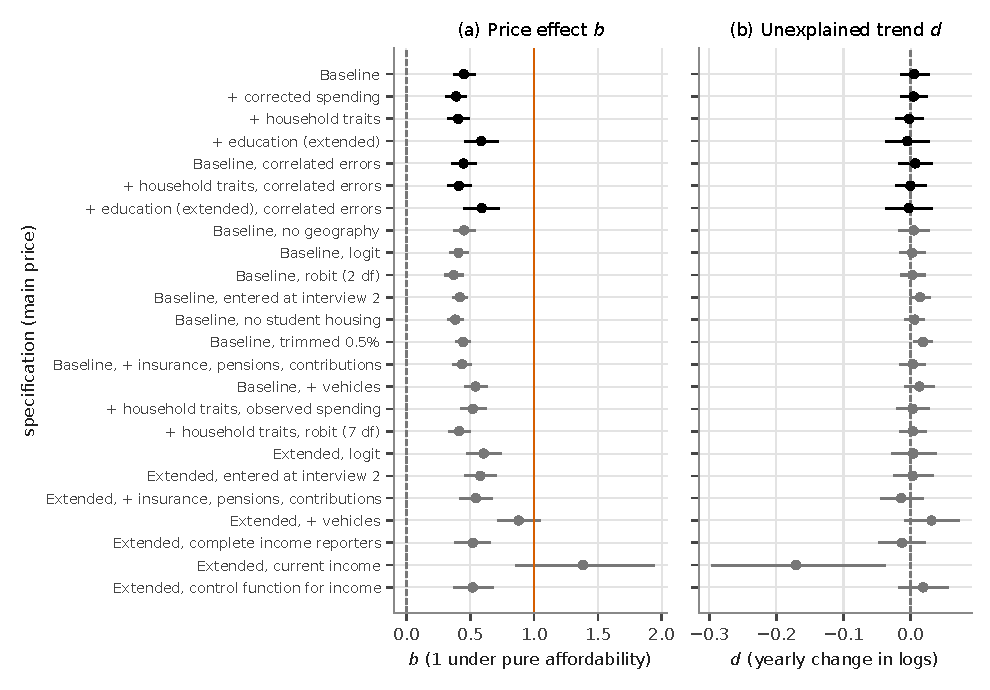
\includegraphics[width=\textwidth]{figures/b_and_d.pdf}
\caption{The price effect $b$ and the unexplained trend $d$ in every specification, main computer price: posterior medians and 90\% intervals. Black: the four CE regressions of 1994--2013, from the baseline to the extended regression, with independent and with correlated sampling errors. Grey: checks. Pure affordability is $b = 1$ (solid vertical line in panel a) and $d = 0$. Dashed lines mark zero.}
\label{fig:bd}
\end{figure}

\subsection{Other computer prices}
\label{app:prices}

Table~\ref{tab:concepts} repeats the second stage under every computer price concept. The two other BEA indexes give similar results, with $b$ between 0.39 and 0.79 and unexplained trends between $-0.030$ and $-0.009$ a year. The unexplained trends under the two other BEA indexes are all negative, because these two indexes fell less than the main index and so leave more of the fall in the spending threshold to the unexplained trend.

The CPI-U for personal computers gives $b = 0.63$ in the baseline regression and 0.93 in the extended regression, with a positive unexplained trend (extended regression: $0.056$ $[0.005, 0.106]$). The difference from the main index reflects the shorter period that the CPI-U covers, 1999 to 2013. The CPI-U and the main index both fall by 0.18 a year in logs from 1999 to 2012, and over those years the computer price falls at an almost constant rate, so the CPI-U fits cannot separate $b$ from $d$ (posterior correlation 0.98).

\begin{table}[p]
\centering
\caption{Second stage under every computer price concept: posterior medians with 90\% intervals. $\Delta\ell$ is the change in the log computer price from the first year used to 2012. The CPI-U starts in 1999.}
\label{tab:concepts}
\footnotesize
\begin{tabular}{lccccc}
\toprule
Specification & Years & $\Delta\ell$ to 2012 & $b$ & $d$ & $\omega$ \\
\midrule
\multicolumn{6}{l}{\textit{BEA PCE, personal computers (main)}} \\
Baseline & 1994--2013 & $-$4.02 & 0.45 [0.37, 0.54] & +0.005 [$-$0.016, +0.028] & 0.029 \\
+ corrected spending & 1994--2013 & $-$4.02 & 0.39 [0.31, 0.47] & +0.005 [$-$0.015, +0.026] & 0.034 \\
+ household traits & 1994--2013 & $-$4.02 & 0.41 [0.32, 0.49] & $-$0.002 [$-$0.023, +0.019] & 0.043 \\
+ education (extended) & 1994--2013 & $-$4.02 & 0.59 [0.46, 0.72] & $-$0.005 [$-$0.037, +0.029] & 0.062 \\
\addlinespace
\multicolumn{6}{l}{\textit{BEA PCE, information processing equipment}} \\
Baseline & 1994--2013 & $-$3.30 & 0.45 [0.36, 0.56] & $-$0.014 [$-$0.034, +0.006] & 0.045 \\
+ corrected spending & 1994--2013 & $-$3.30 & 0.39 [0.30, 0.49] & $-$0.012 [$-$0.032, +0.007] & 0.047 \\
+ household traits & 1994--2013 & $-$3.30 & 0.40 [0.30, 0.51] & $-$0.021 [$-$0.041, $-$0.001] & 0.055 \\
+ education (extended) & 1994--2013 & $-$3.30 & 0.59 [0.43, 0.76] & $-$0.030 [$-$0.063, +0.004] & 0.079 \\
\addlinespace
\multicolumn{6}{l}{\textit{BEA investment, computers}} \\
Baseline & 1994--2013 & $-$2.53 & 0.62 [0.47, 0.77] & $-$0.011 [$-$0.034, +0.014] & 0.058 \\
+ corrected spending & 1994--2013 & $-$2.53 & 0.53 [0.39, 0.67] & $-$0.009 [$-$0.031, +0.012] & 0.056 \\
+ household traits & 1994--2013 & $-$2.53 & 0.54 [0.37, 0.70] & $-$0.019 [$-$0.044, +0.006] & 0.069 \\
+ education (extended) & 1994--2013 & $-$2.53 & 0.79 [0.55, 1.04] & $-$0.027 [$-$0.063, +0.012] & 0.096 \\
\addlinespace
\multicolumn{6}{l}{\textit{BLS CPI-U, personal computers}} \\
Baseline & 1999--2013 & $-$2.36 & 0.63 [0.44, 0.79] & +0.038 [+0.001, +0.070] & 0.023 \\
+ corrected spending & 1999--2013 & $-$2.36 & 0.56 [0.39, 0.70] & +0.034 [+0.003, +0.064] & 0.020 \\
+ household traits & 1999--2013 & $-$2.36 & 0.61 [0.42, 0.77] & +0.034 [$-$0.003, +0.065] & 0.033 \\
+ education (extended) & 1999--2013 & $-$2.36 & 0.93 [0.67, 1.18] & +0.056 [+0.005, +0.106] & 0.043 \\
\addlinespace
\multicolumn{6}{l}{\textit{CE price paid, median}} \\
Baseline & 1994--2013 & $-$0.08 & 0.75 [0.55, 0.96] & $-$0.087 [$-$0.095, $-$0.079] & 0.066 \\
+ corrected spending & 1994--2013 & $-$0.08 & 0.65 [0.47, 0.84] & $-$0.075 [$-$0.082, $-$0.068] & 0.062 \\
+ household traits & 1994--2013 & $-$0.08 & 0.67 [0.48, 0.86] & $-$0.084 [$-$0.091, $-$0.078] & 0.063 \\
+ education (extended) & 1994--2013 & $-$0.08 & 0.96 [0.67, 1.27] & $-$0.123 [$-$0.134, $-$0.111] & 0.094 \\
\addlinespace
\multicolumn{6}{l}{\textit{CE price paid, 90th percentile}} \\
Baseline & 1994--2013 & $-$0.64 & 0.77 [$-$0.07, 1.59] & $-$0.063 [$-$0.103, $-$0.025] & 0.140 \\
+ corrected spending & 1994--2013 & $-$0.64 & 0.68 [$-$0.09, 1.41] & $-$0.054 [$-$0.090, $-$0.019] & 0.123 \\
+ household traits & 1994--2013 & $-$0.64 & 0.80 [$-$0.02, 1.56] & $-$0.059 [$-$0.097, $-$0.022] & 0.124 \\
+ education (extended) & 1994--2013 & $-$0.64 & 1.08 [0.09, 2.06] & $-$0.089 [$-$0.136, $-$0.041] & 0.172 \\
\bottomrule
\end{tabular}

\end{table}

\subsection{Pure affordability predicts a faster spread of computers than occurred}
\label{app:pure}

Against the main computer price, pure affordability overpredicts both the fall in the spending threshold and the rise in the computer ownership rate. The gap from pure affordability, $L_t$ (Appendix~\ref{app:summaries}), reaches 1.79 to 2.57 by 2012 (extended regression: 1.79, SE 0.17). The log spending threshold fell 1.8 to 2.6 less than the log computer price, so by 2012 the spending threshold was 6 to 13 times the level that pure affordability predicts. For the computer ownership rate, the fitted 1994 probit model, applied to 2012 households at the 2012 computer price, predicts a rise 1.29 to 1.34 times the actual rise ($S_{2012}$). That prediction implies that nearly every household owned a computer by 2012, against the actual 81\%. Spending growth alone accounts for 20--25\% of the actual rise ($S^{\text{spend}}_{2012}$ of 0.20 to 0.25), in current dollars, which count general inflation as spending growth. Section~\ref{sec:split} splits the rise between the computer price and household spending at the estimated $b$ and in constant dollars.

\subsection{No other interaction between the computer price and income}
\label{app:nointeraction}

The household model allows no other interaction between the computer price and household income. The computer price and household spending enter the household model only through $x_{it} - b\,\ell_t$, so a fall in the computer price is worth the same rise in spending at every level of income. If the response to the computer price depended on income in some other way, for example through a term $\eta\,x_{it}\,\ell_t$ inside $\Phi$, the spending slope, which is the coefficient on log spending inside $\Phi$, would change as the computer price fell, from $1/\sigma$ to $1/\sigma + \eta\,\ell_t$. Computer prices vary only by year, so a spending slope that stays fixed while the computer price falls is the test of this restriction.

We regress $\hat\beta_t$ on $\ell_t$ over 1994--2012 by weighted least squares, with weights $1/\text{se}(\hat\beta_t)^2$ and standard errors scaled up by the residual scatter where the scatter exceeds the replicate errors. Over the 4.02 fall in the log computer price, the estimated change in the spending slope is $-2.9\%$, $-4.6\%$, $-1.8\%$, and $-0.7\%$ of the mean spending slope in the four CE regressions, from the baseline to the extended regression. Every 90\% interval lies between $-12.3\%$ and $+10.4\%$. The data show no interaction beyond the one that the household model builds in, so \emph{a fall in the computer price was worth the same rise in spending at every level of income}.

\subsection{The CPS and the test for a switch at 20--30\% ownership}
\label{sec:cps}

\paragraph{The CPS spending thresholds.} Table~\ref{tab:cps} gives the CPS spending thresholds. The CPS spending thresholds barely move from 1984 to 1989 (11.34 to 11.32), while the log main computer price falls by 0.66, a fall of about half in the computer price. The CPS spending thresholds then fall steadily, to 9.70 in 2003. The 1984 and 1989 spending thresholds are the least precise, with standard errors of 0.131 and 0.115, almost all of which is CPS sampling error.

The CPS spending thresholds do not match the CE spending thresholds in the years that both surveys cover (Table~\ref{tab:validation} and Figure~\ref{fig:cps}). From 1997 to 2003 the CPS spending thresholds fall by 0.67, against 1.38 for the CE spending thresholds, and the gap between the CPS and CE spending thresholds runs from $-0.18$ to $+0.52$, or $-2.9$ to $+4.9$ standard errors. Applying the CPS imputation to CE households shows why the two surveys differ. The spending thresholds of CE households with imputed spending fall by 0.96 from 1997 to 2003, against 1.41 with the same households' corrected spending. The imputation compresses the path of the spending threshold by about a third, toward the middle of the spending distribution.

For a normally distributed $x$ with mean $\mu$ and standard deviation $\sigma_x$, the spending threshold is
\begin{equation}
\tau = \mu - \Phi^{-1}(P)\,\sqrt{1/\beta^2 + \sigma_x^2},
\end{equation}
where $P$ is the computer ownership rate. Imputed spending has a smaller spread and a steeper spending slope than corrected spending ($\hat\beta$ of 0.81 to 0.88, against 0.58 to 0.67). These two changes do not offset each other, as they would under regression calibration, so the distance between the spending threshold and mean spending shrinks. The compression vanishes where the computer ownership rate is near 50\% (2000: 9.99 imputed, 10.00 corrected) and grows as the computer ownership rate moves away from 50\%. A rough reading, which we have not estimated, is that if the CPS path is compressed by the same third, the CPS understates the relation of the spending threshold to the computer price by the same factor.

\begin{figure}[t]
\centering
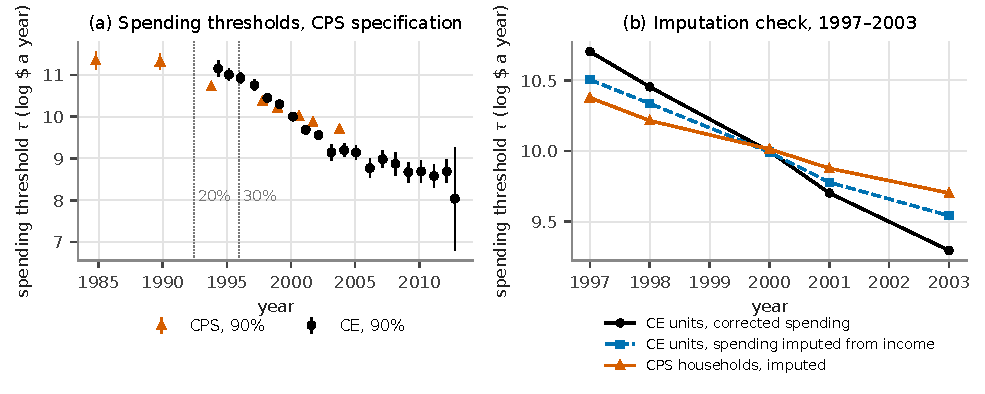
\includegraphics[width=\textwidth]{figures/cps_ce.pdf}
\caption{(a) Spending thresholds from the CPS (imputed long-run spending, eight supplements from October 1984 to October 2003) and the CE (corrected long-run spending, 1994--2013), with the same specification and 90\% intervals, at each survey's date. (b) The imputation check, 1997--2003: spending thresholds of CE households (complete income reporters) with corrected spending and with spending imputed from their income as in the CPS, and the CPS spending thresholds.}
\label{fig:cps}
\end{figure}

\paragraph{A change in the unexplained trend?} Table~\ref{tab:switch} and Figure~\ref{fig:switch} give the results. With both surveys, which together cover 1984 to 2013, the model with a switch at a computer ownership rate of 30\% best predicts the spending thresholds left out of the fit. The 30\% switch model is ahead of the 20\% switch model by 3.8 (SE 2.1) in expected log predictive density (elpd, a measure of how well a model predicts left-out data, where higher is better), and ahead of the one-trend model by 8.7 (SE 4.5). Before late 1995 the spending threshold rose relative to the path that the computer price predicts ($d_1 = 0.052$ $[-0.007, 0.112]$), and after late 1995 the spending threshold fell relative to that path ($d_2 = -0.044$ $[-0.093, 0.008]$), a change of $-0.096$ $[-0.132, -0.060]$ a year, with $b = 0.46$ $[0.27, 0.67]$. The other BEA indexes give the same pattern. Under the 20\% switch model, all but one of the 28 spending thresholds (CPS 1993) lie inside their 90\% posterior predictive intervals.

We do not believe that the switch at 30\% is real. The switch date falls where the data change from the CPS, which supplies most of the spending thresholds before the switch date, to the CE, which supplies most of the spending thresholds after the switch date. The comparison above showed that the CPS path is compressed where the two surveys overlap, and the same compression before 1997 would make the CPS spending thresholds before the switch date fall too slowly. The spending thresholds from the two surveys also do not lie on one path. Under the main computer price, the combined fits need year-specific deviations with a standard deviation of 0.15 to 0.21, against 0.014 to 0.019 for the CPS alone. And within the CPS alone, which is the one survey that measures computer ownership consistently across both switch dates, the model with one unexplained trend predicts best, ahead of the 30\% switch model by 2.1 (SE 0.6). Within the CPS, the change in the unexplained trend is $-0.005$ $[-0.038, 0.037]$ at 30\% and $0.013$ $[-0.050, 0.079]$ at 20\%, and the one-trend model gives $b = 0.32$ $[0.15, 0.49]$ and $d = -0.012$ $[-0.062, 0.036]$.

Only the 1984 and 1989 surveys lie below a computer ownership rate of 20\%, and both surveys have the largest standard errors, so the surveys contain little information about a switch at 20\%. The early phase of the spread of computers is where the profit switch hypothesis is most distinctive, and the surveys have the fewest observations in that early phase.

\begin{table}[t]
\centering
\caption{The switch test, CPS (October 1984 to October 2003) and CE (1994--2013): posterior medians with 90\% intervals. $d_1$ and $d_2$ are the unexplained trends before and after the switch date (yearly changes in the log spending threshold), and $o$ is the CPS offset. $\Delta\widehat{\text{elpd}}$ is the difference in expected log predictive density from the best model in its panel, with its standard error (leave-one-out, with exact refits for Pareto $k > 0.7$).}
\label{tab:switch}
\resizebox{\textwidth}{!}{\scriptsize
\begin{tabular}{lccccccc}
\toprule
Model & $b$ & $d_1$ (one trend: $d$) & $d_2$ & $d_2-d_1$ & $o$ & $\omega$ & $\Delta\widehat{\mathrm{elpd}}$ (SE) \\
\midrule
\multicolumn{8}{l}{\textit{CPS and CE spending thresholds, with a CPS offset (the approved model)}} \\
One trend & 0.46 [0.20, 0.72] & $-$0.023 [$-$0.087, +0.041] &  &  & +0.01 [$-$0.16, +0.19] & 0.212 & $-$8.7 (4.5) \\
Switch at 20\% & 0.39 [0.17, 0.61] & +0.065 [$-$0.004, +0.134] & $-$0.056 [$-$0.110, +0.001] & $-$0.121 [$-$0.176, $-$0.064] & +0.04 [$-$0.11, +0.18] & 0.169 & $-$3.8 (2.1) \\
Switch at 30\% & 0.46 [0.27, 0.67] & +0.052 [$-$0.007, +0.112] & $-$0.044 [$-$0.093, +0.008] & $-$0.096 [$-$0.132, $-$0.060] & +0.07 [$-$0.07, +0.20] & 0.150 & 0 (best) \\
\addlinespace
\multicolumn{8}{l}{\textit{CPS spending thresholds alone (check)}} \\
One trend & 0.32 [0.15, 0.49] & $-$0.012 [$-$0.062, +0.036] &  &  &  & 0.014 & 0 (best) \\
Switch at 20\% & 0.38 [0.04, 0.75] & $-$0.005 [$-$0.065, +0.057] & +0.006 [$-$0.098, +0.122] & +0.013 [$-$0.050, +0.079] &  & 0.019 & $-$2.8 (1.4) \\
Switch at 30\% & 0.30 [0.06, 0.57] & $-$0.015 [$-$0.072, +0.047] & $-$0.020 [$-$0.095, +0.069] & $-$0.005 [$-$0.038, +0.037] &  & 0.017 & $-$2.1 (0.6) \\
\bottomrule
\end{tabular}
}
\end{table}

\begin{figure}[t]
\centering
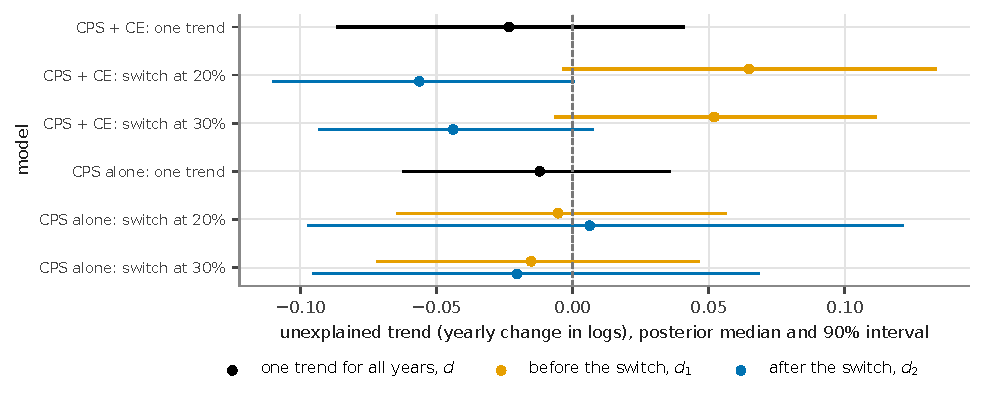
\includegraphics[width=\textwidth]{figures/switch.pdf}
\caption{Unexplained trend before and after the switch date, main computer price: posterior medians and 90\% intervals. CPS + CE: the switch test with a CPS offset, 1984--2013. CPS alone: the check on the CPS spending thresholds, October 1984 to October 2003.}
\label{fig:switch}
\end{figure}

\subsection{One joint model gives the same answer}
\label{sec:joint}

The joint model matches the two-stage estimates of the extended regression (Table~\ref{tab:joint} and Figure~\ref{fig:joint}). The joint model gives $b = 0.60$ $[0.45, 0.74]$ against 0.59 $[0.46, 0.72]$ from the two stages, and $d = -0.003$ $[-0.038, 0.029]$ against $-0.005$ $[-0.037, 0.029]$, with the same posterior correlation of $b$ and $d$ (0.97). From 1994 to 2012 the joint model's spending thresholds differ from the extended regression's first-stage spending thresholds by at most 0.07 (in 2003), or 0.67 first-stage standard errors, and the joint model's spending slopes $\beta_t$ differ from the first-stage spending slopes by at most 0.04. The differences follow each first-stage spending threshold's distance from the joint model's fitted line (correlation 0.92 over 1994--2012), because the joint model pulls the yearly spending thresholds toward its fitted line, most where the first-stage standard errors are largest. The 2013 spending threshold, which rests on one quarter of data, moves from 8.10 to 8.58, or 0.68 standard errors. Over all 1{,}027 parameters and derived quantities, $\hat R \le 1.008$, bulk and tail effective sample sizes are at least 1{,}532 and 1{,}779, and there are no divergent transitions.

The joint model's intervals for $b$ and $d$ are no narrower than the two-stage intervals. The joint model's year-specific deviations are larger ($\omega = 0.089$ against 0.062), which offsets the joint model's narrower intervals for the yearly spending thresholds. Those narrower intervals are partly an artefact.

The joint model's pseudo-likelihood understates the sampling error of the spending thresholds \citep{williams2021}. Each year's fit on its own, with households treated as independent, gives standard errors of $\tau_t$ of 0.57 to 0.96 times the replicate standard errors in 1994--2012 (median 0.75). A sandwich estimator that allows for unequal weights gives 0.65 to 1.09 times the replicate standard errors (median 0.82), so the rest of the gap reflects the survey's strata and clusters and the spending correction, which the joint model treats as known. Pooling the years toward the fitted line narrows the joint model's 90\% intervals for $\tau_t$ further, to 0.47 to 0.86 times the width of the replicate intervals. The understated sampling error also inflates $\omega$, because the joint model attributes to year-specific deviations what the replicate standard errors attribute to sampling error. The joint model's intervals therefore do not reflect the survey design, and the comparison of the joint model with the two-stage fit is a comparison of point estimates.

\begin{table}[t]
\centering
\caption{The joint model against the two-stage estimates (extended regression, main computer price, CE households of 1994--2013): posterior medians with 90\% intervals. The joint model's intervals do not allow for the survey design (see text).}
\label{tab:joint}
\footnotesize
\begin{tabular}{lcc}
\toprule
Parameter & Joint model & Two-stage (extended regression) \\
\midrule
$a$ & 11.14 [11.04, 11.24] & 11.15 [11.05, 11.23] \\
$b$ & 0.60 [0.45, 0.73] & 0.59 [0.46, 0.72] \\
$d$ & $-$0.003 [$-$0.038, +0.028] & $-$0.005 [$-$0.037, +0.029] \\
$\omega$ & 0.090 [0.059, 0.139] & 0.062 [0.028, 0.108] \\
\bottomrule
\end{tabular}

\end{table}

\begin{figure}[t]
\centering
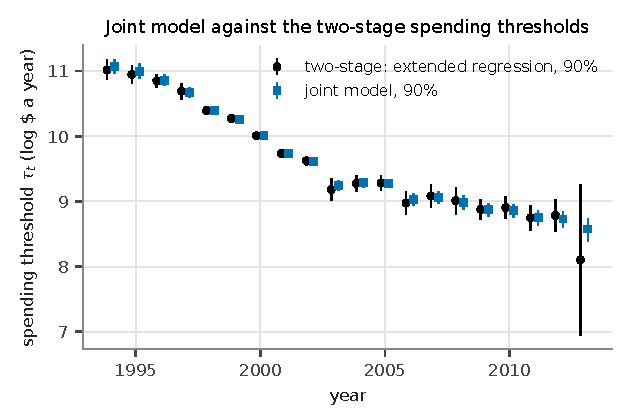
\includegraphics{figures/joint.pdf}
\caption{Yearly spending thresholds, 1994--2013, from the joint model (posterior medians with 90\% intervals) and from the first stage of the extended regression ($\pm 1.645$ replicate standard errors). The joint model's intervals do not allow for the survey design.}
\label{fig:joint}
\end{figure}

\section{Departures from the analysis plan}
\label{app:deviations}

The analysis plan numbered the regressions as seven steps, and the code keeps those numbers. Step 1 is the baseline regression. Steps 2--4 add the three parts of the extended regression one at a time, steps 5 and 6 are the CPS extension, and step 7 is the joint model.

The cross-validation rule set before estimation picks a robit model with 2 degrees of freedom for the baseline regression and a robit model with 7 degrees of freedom for the regression with household traits but no education. We kept the probit model throughout, so that every regression, the second stage, and the joint model share one link function, and we report the rule's link functions as checks. The robit link functions change the price effect little, with $b = 0.37$ $[0.30, 0.45]$ against 0.45 in the baseline regression, and $0.41$ $[0.33, 0.50]$ against 0.41 with household traits.

The analysis plan placed the date at which the computer ownership rate passed 20\% in mid-1991. Interpolation between the CPS surveys puts that date in spring 1992 (1992.30 to 1992.44), and the switch test uses 1992.44.

The full set of checks runs on the baseline and extended regressions, which bracket the two intermediate regressions, since the extended regression contains every change that the intermediate regressions make. The regression with household traits but no education has only the observed-spending and robit-model checks, and the regression with corrected spending alone has no checks of its own. The CPS spending thresholds have no link or weighting checks, since the income imputation is what limits the CPS spending thresholds.

The CPS sampling error assumes a design effect of 2, since the public CPS files of these years carry no replicate weights or design codes.

The analysis plan expected the imputed CPS spending thresholds to match the CE spending thresholds in the years that both surveys cover. The CPS spending thresholds do not match the CE spending thresholds (Appendix~\ref{sec:cps}), so the switch test adds the CPS-alone check, and we read the combined CPS and CE results as an artefact of combining the two surveys.

The joint model samples in QR coordinates centred at each year's own fit. We made this change of variables because the direct parametrization reached the sampler's maximum tree depth in pilots on a 5\% subsample, and a pilot on all households had not finished its 300 warm-up iterations after 14 minutes. In the rotated coordinates the sampler needs 31 leapfrog steps per iteration (tree depth 5). The joint model's geography prior applies to effects constrained by the pooled shares, whereas the first stage puts the same prior on unconstrained effects next to a free intercept. Each year's fit under the joint model's priors reproduces the extended regression's spending thresholds to within 0.004 in logs and the spending slopes to within 0.003, so this difference in priors is immaterial. The joint model's intervals do not allow for the survey design (Appendix~\ref{sec:joint}).

Sections~\ref{sec:split} and~\ref{sec:interaction}, on household spending, the computer price, and their interaction, are additions to the analysis plan. Both sections use only estimates that the plan already produces (the baseline regression's fits and second stage), and their intervals allow for the uncertainty in $b$ only. The constant-dollar version of the second stage in the four CE regressions is also an addition. The constant-dollar version leaves the approved current-dollar estimates unchanged.

\section{Reproduction}

\begingroup\raggedright
The code, the processed data, and this paper are at \url{https://github.com/IlanStrauss/home-computer-diffusion}. The repository's \texttt{README.md} explains how to download the raw survey files and gives the full run order, and \texttt{run\_all.sh} runs every script in that order. After the build scripts, the run order is \texttt{explore\_data.py}, \texttt{link\_choice.py}, \texttt{first\_stage.py}, \texttt{second\_stage.R}, \texttt{second\_stage\_constant.R}, \texttt{income\_price.py}, \texttt{education\_raw\_gap.py}, \texttt{cps\_extension.py}, \texttt{cps\_switch.R 1992.44 1995.96}, \texttt{joint\_prepare.py}, \texttt{joint\_model.py}, and \texttt{joint\_design\_effect.py}, all in \texttt{code/}. Each script writes a log to \texttt{output/logs/}, and the estimates go to \texttt{output/results/}. Then \texttt{figures.py} and \texttt{tables.py} write the figures and tables that this paper inputs. For readers who want the data without the model, \texttt{build\_combined.py} writes \texttt{households\_combined.csv.gz}, which holds the 178{,}891 CE households of January 1994 to March 2013 and the 425{,}627 CPS households of October 1984 to October 2003 in one file, with common variable names and codes and the BEA computer price index for the month of each household's computer answer.\par
\endgroup

\section{Appendix tables}

\begin{table}[h]
\centering
\caption{Cross-validated log score of each link function (10-fold within each year, weighted, summed over 1994--2013): difference from the probit link, with its standard error. Higher is better.}
\label{tab:links}
\footnotesize
\begin{tabular}{lccc}
\toprule
Link & Baseline (geography) & + household traits & + education (extended) \\
\midrule
Probit & 0 & 0 & 0 \\
Logit & +273.6 (19.5) & +62.6 (15.6) & +21.9 (14.4) \\
Robit, 7 df & +281.0 (20.9) & +70.6 (16.5) & +26.9 (14.8) \\
Robit, 4 df & +411.2 (30.3) & +55.7 (24.5) & $-$25.6 (23.0) \\
Robit, 2 df & +567.5 (45.8) & $-$101.8 (39.0) & $-$289.4 (38.2) \\
\bottomrule
\end{tabular}

\end{table}

\begin{table}[h]
\centering
\caption{CPS spending thresholds (imputed long-run spending, CPS specification). Date is the survey month in decimal years. The households and computer ownership rates are those in the fit (households with a known income bracket and traits), so the computer ownership rates differ from the shares of all answering households in Appendix~\ref{app:data}. SE combines mapping and sampling error. $\ell$ is the main log computer price relative to the CE's 1994 average.}
\label{tab:cps}
\footnotesize
\begin{tabular}{rcrrcccc}
\toprule
Year & Date & Households & Own (\%) & $\hat\tau$ & SE & $\hat\beta$ & $\ell$ \\
\midrule
1984 & 1984.79 & 51,162 & 8.2 & 11.34 & 0.131 & 0.92 & 1.61 \\
1989 & 1989.79 & 50,475 & 15.2 & 11.32 & 0.115 & 0.78 & 0.95 \\
1993 & 1993.79 & 50,886 & 23.5 & 10.73 & 0.044 & 1.06 & 0.08 \\
1997 & 1997.79 & 42,458 & 38.2 & 10.38 & 0.022 & 1.10 & $-$1.12 \\
1998 & 1998.96 & 41,618 & 44.1 & 10.21 & 0.015 & 1.14 & $-$1.59 \\
2000 & 2000.62 & 40,011 & 53.4 & 10.01 & 0.011 & 1.23 & $-$2.10 \\
2001 & 2001.71 & 47,351 & 59.0 & 9.88 & 0.014 & 1.21 & $-$2.45 \\
2003 & 2003.79 & 45,432 & 64.4 & 9.70 & 0.022 & 1.09 & $-$2.95 \\
\bottomrule
\end{tabular}

\end{table}

\begin{table}[h]
\centering
\caption{The CPS against the CE in the five years that both surveys cover (1997, 1998, 2000, 2001, and 2003). Left: CPS against CE spending thresholds from the same specification (CE interpolated to the CPS month). Right: CE households (complete income reporters) fitted with spending imputed from income, with corrected spending, and with observed spending (point estimates).}
\label{tab:validation}
\resizebox{\textwidth}{!}{\footnotesize
\begin{tabular}{rccccccccc}
\toprule
& \multicolumn{4}{c}{CPS against CE} & \multicolumn{5}{c}{CE households, same year} \\
\cmidrule(lr){2-5}\cmidrule(lr){6-10}
Year & CPS $\hat\tau$ & CE $\hat\tau$ & Gap & Gap/SE & $\hat\tau$ imputed & $\hat\tau$ corrected & $\hat\tau$ observed & $\hat\beta$ imputed & $\hat\beta$ corrected \\
\midrule
1997 & 10.38 & 10.56 & $-$0.18 & $-$2.9 & 10.50 & 10.70 & 10.85 & 0.88 & 0.67 \\
1998 & 10.21 & 10.32 & $-$0.11 & $-$2.9 & 10.34 & 10.45 & 10.55 & 0.84 & 0.66 \\
2000 & 10.01 & 9.85 & +0.16 & +4.1 & 9.99 & 10.00 & 9.99 & 0.83 & 0.61 \\
2001 & 9.88 & 9.61 & +0.26 & +4.9 & 9.78 & 9.70 & 9.62 & 0.82 & 0.64 \\
2003 & 9.70 & 9.18 & +0.52 & +4.9 & 9.54 & 9.30 & 9.14 & 0.81 & 0.58 \\
\bottomrule
\end{tabular}
}
\end{table}

\begin{table}[p]
\centering
\caption{Yearly spending thresholds $\hat\tau_t$, the log long-run spending at which a household with average location and traits has a 50\% chance of owning a computer (replicate standard errors), and spending slopes $\hat\beta_t$, from the baseline regression to the extended regression. $\ell_t$ is the main log computer price relative to 1994. 2013 has the first quarter only.}
\label{tab:thresholds}
\resizebox{\textwidth}{!}{\scriptsize
\begin{tabular}{rrrrcccccccc}
\toprule
Year & Households & Own (\%) & $\ell_t$ & \multicolumn{2}{c}{Baseline} & \multicolumn{2}{c}{+ corrected spending} & \multicolumn{2}{c}{+ household traits} & \multicolumn{2}{c}{+ education (extended)} \\
\cmidrule(lr){5-6}\cmidrule(lr){7-8}\cmidrule(lr){9-10}\cmidrule(lr){11-12}
 & & & & $\hat\tau_t$ (SE) & $\hat\beta_t$ & $\hat\tau_t$ (SE) & $\hat\beta_t$ & $\hat\tau_t$ (SE) & $\hat\beta_t$ & $\hat\tau_t$ (SE) & $\hat\beta_t$ \\
\midrule
1994 & 9,966 & 23.8 & 0.00 & 10.81 (0.05) & 0.83 & 10.72 (0.05) & 0.91 & 10.73 (0.06) & 0.96 & 11.02 (0.09) & 0.72 \\
1995 & 6,153 & 26.6 & $-$0.17 & 10.66 (0.04) & 0.87 & 10.54 (0.04) & 1.04 & 10.66 (0.05) & 0.99 & 10.95 (0.09) & 0.73 \\
1996 & 9,664 & 30.8 & $-$0.46 & 10.61 (0.03) & 0.75 & 10.53 (0.03) & 0.86 & 10.59 (0.03) & 0.90 & 10.85 (0.06) & 0.65 \\
1997 & 7,020 & 35.2 & $-$0.87 & 10.45 (0.03) & 0.83 & 10.41 (0.02) & 0.92 & 10.48 (0.04) & 0.94 & 10.69 (0.07) & 0.68 \\
1998 & 7,023 & 40.8 & $-$1.27 & 10.26 (0.02) & 0.83 & 10.23 (0.02) & 0.92 & 10.28 (0.02) & 1.01 & 10.40 (0.04) & 0.77 \\
1999 & 11,003 & 44.5 & $-$1.64 & 10.16 (0.02) & 0.83 & 10.14 (0.02) & 0.93 & 10.20 (0.02) & 0.92 & 10.27 (0.03) & 0.70 \\
2000 & 9,725 & 50.1 & $-$1.97 & 9.98 (0.02) & 0.82 & 9.98 (0.02) & 0.92 & 10.02 (0.02) & 0.96 & 10.01 (0.02) & 0.72 \\
2001 & 9,436 & 56.9 & $-$2.28 & 9.76 (0.04) & 0.79 & 9.80 (0.04) & 0.89 & 9.83 (0.02) & 0.94 & 9.74 (0.03) & 0.69 \\
2002 & 9,969 & 60.3 & $-$2.58 & 9.67 (0.04) & 0.82 & 9.71 (0.04) & 0.93 & 9.73 (0.03) & 0.97 & 9.62 (0.04) & 0.76 \\
2003 & 10,246 & 64.2 & $-$2.83 & 9.45 (0.08) & 0.70 & 9.52 (0.07) & 0.79 & 9.46 (0.06) & 0.74 & 9.18 (0.10) & 0.52 \\
2004 & 9,936 & 67.9 & $-$3.00 & 9.45 (0.06) & 0.84 & 9.52 (0.05) & 0.94 & 9.48 (0.05) & 0.92 & 9.28 (0.08) & 0.71 \\
2005 & 13,743 & 68.5 & $-$3.15 & 9.44 (0.04) & 0.78 & 9.52 (0.04) & 0.88 & 9.52 (0.04) & 0.94 & 9.28 (0.07) & 0.71 \\
2006 & 9,248 & 71.6 & $-$3.33 & 9.38 (0.06) & 0.77 & 9.47 (0.06) & 0.86 & 9.38 (0.06) & 0.85 & 8.98 (0.11) & 0.60 \\
2007 & 8,680 & 73.9 & $-$3.46 & 9.41 (0.07) & 0.85 & 9.50 (0.06) & 0.94 & 9.42 (0.06) & 0.95 & 9.08 (0.11) & 0.70 \\
2008 & 8,976 & 75.8 & $-$3.59 & 9.35 (0.09) & 0.86 & 9.45 (0.08) & 0.95 & 9.38 (0.07) & 0.96 & 9.01 (0.13) & 0.71 \\
2009 & 9,098 & 77.3 & $-$3.73 & 9.17 (0.09) & 0.78 & 9.28 (0.08) & 0.87 & 9.24 (0.06) & 0.93 & 8.88 (0.10) & 0.70 \\
2010 & 9,214 & 79.3 & $-$3.83 & 9.12 (0.09) & 0.81 & 9.23 (0.08) & 0.91 & 9.25 (0.06) & 1.03 & 8.90 (0.10) & 0.78 \\
2011 & 8,809 & 80.4 & $-$3.92 & 9.12 (0.10) & 0.83 & 9.24 (0.09) & 0.92 & 9.13 (0.07) & 0.95 & 8.75 (0.12) & 0.73 \\
2012 & 8,779 & 80.5 & $-$4.02 & 9.16 (0.08) & 0.84 & 9.27 (0.07) & 0.94 & 9.13 (0.08) & 0.94 & 8.78 (0.15) & 0.72 \\
2013 & 2,203 & 80.6 & $-$4.08 & 8.82 (0.22) & 0.65 & 8.99 (0.19) & 0.74 & 8.71 (0.27) & 0.70 & 8.10 (0.70) & 0.50 \\
\bottomrule
\end{tabular}
}
\end{table}

\end{document}
